%% ============================================================================
%% Sensitivity of 2D flood models to Manning roughness uncertainty:
%% a Monte Carlo comparison of SFINCS and HEC-RAS in the Besaya River
%% ============================================================================
\documentclass[review,12pt]{elsarticle}

\usepackage[utf8]{inputenc}
\usepackage[T1]{fontenc}
\usepackage{amsmath,amssymb}
\usepackage{graphicx}
\usepackage{booktabs}
\usepackage{array}
\usepackage{multirow}
\usepackage{siunitx}
\usepackage{natbib}
\usepackage[colorlinks=true,linkcolor=black,citecolor=black,urlcolor=blue]{hyperref}
\usepackage{xcolor}
\usepackage{lineno}
\usepackage{setspace}
\usepackage{microtype}
\usepackage{pdflscape}
\usepackage[margin=2.5cm]{geometry}

\linenumbers
\doublespacing

\journal{Journal of Hydrology}

\bibliographystyle{elsarticle-harv}

% convenience macros
\newcommand{\nman}{$n$}
\newcommand{\CV}{\text{CV}}
\newcommand{\sfincs}{\textsc{SFINCS}}
\newcommand{\hecras}{\textsc{HEC-RAS}}

%% ===========================================================================
\begin{document}

\begin{frontmatter}

\title{Sensitivity of two-dimensional flood inundation models to Manning
roughness uncertainty: a Monte Carlo comparison of \sfincs{} and \hecras{}
in the Besaya River floodplain (northern Spain)}

\author[hl]{Salvador Navas\corref{cor1}}
\ead{salvador.navas@hidralab.com}

\author[uclm]{\'Alvaro Gal\'an}

\author[uc]{Manuel del Jesus}

\cortext[cor1]{Corresponding author}

\address[hl]{HidraLab, Avda.\ Camilo Jos\'e Cela s/n, 13005 Ciudad Real, Spain}

\address[uclm]{Escuela T\'ecnica Superior de Ingenier\'ia de Caminos, Canales y Puertos,
Universidad de Castilla-La Mancha, Avda.\ Camilo Jos\'e Cela s/n,
13071 Ciudad Real, Spain}

\address[uc]{Escuela T\'ecnica Superior de Ingenieros de Caminos, Canales y Puertos,
Universidad de Cantabria, Avda.\ de los Castros s/n, 39005 Santander, Spain}

%% ---------------------------------------------------------------------------
\begin{abstract}
Manning's roughness coefficient \nman{} is a primary source of parametric
uncertainty in two-dimensional flood inundation models, yet its aggregate
effect on model outputs is rarely quantified across hydraulically distinct
model formulations subjected to the same stochastic input ensemble.
This study performs a systematic Monte Carlo sensitivity analysis
(\num{1000} simulations; \num{9} land use classes) of Manning uncertainty
in two widely used 2D hydraulic models --- \sfincs{} (simplified inertial
equations) and \hecras{} 6.6 (full 2D Saint-Venant equations) --- applied to
the Besaya River at Corrales de Buelna (Cantabria, northern Spain) under
a 500-year return period flood event.
For each land use class, candidate parametric distributions are fitted to
bibliographic roughness ranges (4--9 values per class; median: 6) via
Kolmogorov--Smirnov selection tests, and \num{1000} independent Manning
combination vectors are drawn by Monte Carlo sampling from a pool of
\num{10000} realizations per class.
Flood outputs (spatially averaged water depth and inundated area) are compared
between models using Pearson correlation, systematic bias, root mean square
error and coefficient of variation.
Five simulations (0.5\%) identified as numerical non-convergences via
robust $z$-scores are removed, leaving $N = 995$ valid simulation pairs.

Results reveal that the spatially averaged wet-cell Manning coefficient
explains less than 2\% of the variance in domain-scale flood outputs
in both models ($r^2 < 0.02$), with
ensemble coefficients of variation ranging from 2.0\% to 8.4\%.
\hecras{} is significantly more sensitive to Manning uncertainty than
\sfincs{} (CV\textsubscript{area} = 8.4\% vs.\ 2.0\%; regression slope
$\partial\bar{h}/\partial n$ is $6\times$ larger), and produces a
systematic positive bias relative to \sfincs{} ($+0.17$~m depth;
$+0.15$~km\textsuperscript{2} area).
The simulation-to-simulation correlation between the two models is only
moderate ($r = 0.52$ for depth; $r = 0.49$ for area), indicating that
model-structure uncertainty exceeds Manning parametric uncertainty.
Critically, the flooded-area distribution of \hecras{} is \emph{bimodal}:
90\% of simulations cluster in a high-area regime
($\bar{A} = 0.700$~km\textsuperscript{2}) and 10\% in a low-area regime
($\bar{A} = 0.577$~km\textsuperscript{2}), corresponding to two distinct
horizontal bands in the Manning--area scatter plot.
Spatial frequency analysis and topographic corridor analysis reveal that
this bimodality is governed by a topographic saddle at
$z = 60.1$~m~a.s.l.\ controlling hydraulic access to a secondary
floodplain of 7.4~ha.
The advective momentum terms retained in the full Saint-Venant equations
are the proposed mechanism enabling \hecras{} to resolve directional
inertial momentum transfer towards the saddle, triggering the abrupt
transition to the high-area regime when the threshold is marginally exceeded.
The simplified inertial formulation of \sfincs{}, which omits the advective
acceleration term, produces a smooth unimodal response with no such bifurcation.
No individual Manning coefficient, nor the spatially averaged wet-cell Manning
value $\bar{n}$, predicts which regime a simulation will enter
(all Spearman $|\rho| < 0.03$, $p > 0.35$; Pearson $|r| < 0.06$, $p > 0.05$),
supporting the interpretation
that the bifurcation is a compound non-linear effect associated with model
structure rather than with any specific land use roughness class.
These findings demonstrate that model-structure choice introduces qualitative
changes in the uncertainty distribution of flood outputs --- not merely
scalar offsets in mean values --- with direct implications for probabilistic
flood hazard mapping, model ensemble design and the identification of
topographic tipping points in floodplain systems.
\end{abstract}

\begin{keyword}
Manning roughness \sep Monte Carlo sensitivity analysis \sep
2D flood modelling \sep \textsc{SFINCS} \sep \textsc{HEC-RAS} \sep
hydraulic bifurcation \sep model-structure uncertainty \sep
topographic threshold \sep floodplain inundation \sep Spain
\end{keyword}

\end{frontmatter}

%% ===========================================================================
\section{Introduction}
\label{sec:intro}

Flood inundation modelling is central to modern flood risk management, forming
the basis for hazard mapping, infrastructure design, emergency planning and
the calibration of early-warning systems \citep{teng2017}.
Two-dimensional (2D) shallow-water models have become the operational standard
for this purpose, offering a spatially explicit representation of flow patterns
and inundation extents that one-dimensional approaches cannot capture in
complex floodplain geometries \citep{horritt2002, bates2010}.
Yet model predictions remain subject to multiple interacting sources of
uncertainty, including topographic input errors, boundary condition
specification, numerical discretisation and --- perhaps most pervasively ---
parametric uncertainty in friction coefficients \citep{pappenberger2005,
apel2008, merwade2008}.

Manning's roughness coefficient \nman{} is the dominant hydraulic friction
parameter in open-channel and floodplain flow modelling.
It must be spatially assigned to a heterogeneous land use mosaic on the basis
of classification tables \citep{chow1959, barnes1967, brater1996, fhwa1984}
whose values span wide ranges --- up to an order of magnitude between smooth
channels and densely vegetated floodplains --- and are derived from
field surveys that may not be representative of the study site, flow depth
or seasonal vegetation state.
Because Manning's equation enters the momentum balance as $n^2/h^{4/3}$
in the friction term, roughness uncertainty interacts non-linearly with
water depth, implying that the sensitivity of model outputs to \nman{}
depends on both the magnitude of the uncertainty and the hydraulic conditions
being simulated \citep{hall2005, savage2016}.

Monte Carlo (MC) methods provide a principled framework for uncertainty
propagation that avoids linearisation assumptions inherent in first-order
variance methods \citep{saltelli2010}.
In the MC approach, probability distributions are assigned to uncertain
parameters, random combinations are drawn, and the resulting ensemble of
model outputs is used to characterize output uncertainty.
This approach was pioneered in flood modelling by \citet{aronica2002} and
\citet{pappenberger2005} and has since been applied to quantify the effects
of roughness uncertainty in both 1D and 2D inundation models
\citep{hall2005, mcmillan2010, savage2016, pinos2023, ulate2024}.

A recurrent finding of these studies is that spatially averaged flood outputs
are less sensitive to Manning uncertainty than local metrics such as water
stage at individual cross-sections \citep{pappenberger2005, fewtrell2011},
because spatial aggregation tends to buffer local roughness effects across
the model domain.
However, most existing sensitivity studies are limited to a single model
formulation and rarely address whether the \emph{qualitative structure} of
the output uncertainty distribution --- its shape and potential multimodality ---
depends on the hydraulic equations being solved.

This is a consequential gap because modern flood risk practice increasingly
relies on ensembles of models spanning different complexity levels
\citep{teng2017, vandaele2024, liu2019}.
\sfincs{} \citep{deltares2023sfincs, leijnse2021} and \hecras{}
\citep{usace2021hecras} represent two widely deployed but hydraulically
distinct approaches that are both used operationally for design-flood mapping
and probabilistic hazard assessment.
\sfincs{} solves the simplified inertial (SI) approximation, which retains the
local acceleration and pressure gradient terms of the shallow-water equations
but neglects the advective acceleration $\mathbf{u}\cdot\nabla\mathbf{u}$.
This simplification produces a highly efficient solver suitable for real-time
and large-scale applications \citep{bates2010, neal2012}, but may fail to
capture flow dynamics where inertial momentum transport is significant.
\hecras{} solves the full 2D Saint-Venant equations (SVE), retaining the
advective terms $\rho\mathbf{u}\cdot\nabla\mathbf{u}$, at the cost of
greater computational demand.
The two models have been compared for mean-state predictions in estuarine
\citep{kumbier2019} and riverine \citep{horritt2002} settings, but their
differential sensitivity to Manning parametric uncertainty under identical
boundary conditions and the same stochastic input ensemble has not been
systematically investigated.

A further motivation for this study comes from recent findings that
floodplain topography can create hydraulic tipping points --- threshold
elevations at which small changes in boundary conditions produce abrupt
transitions in inundation extent \citep{apel2008}.
Whether different hydraulic formulations reproduce or mask these thresholds
has important implications for probabilistic flood risk assessment: a model
that smooths a bimodal hazard into a unimodal distribution will systematically
understate the probability of secondary flooding zones.

This study addresses the following research questions:
\begin{enumerate}
  \item How sensitive are \sfincs{} and \hecras{} to Manning roughness
        uncertainty, as quantified by the coefficient of variation and
        regression slope of key flood outputs across a 995-member ensemble?
  \item How consistent are the two models in their simulation-by-simulation
        response to the same Manning perturbation --- i.e., how much of the
        inter-simulation variance is shared?
  \item Does the hydraulic formulation affect the qualitative structure of
        the output uncertainty distribution --- particularly its shape and
        potential multimodality?
  \item What physical mechanism drives any structural differences, and how
        can it be identified from spatial analysis of the flood ensemble?
\end{enumerate}

To answer these questions, we generate 1\,000 Monte Carlo Manning combinations
for nine land use classes, run each combination in both models for a $T = 500$
year design flood in the Besaya River at Corrales de Buelna (Cantabria,
northern Spain), and analyze the resulting ensemble of \num{1990} simulations
using statistical and spatial methods implemented in the open-source
\texttt{pyhydra} Python package.

%% ===========================================================================
\section{Study area}
\label{sec:area}

\subsection{Basin and climate}
\label{sec:basin}

The Besaya River drains a catchment of approximately 680~km\textsuperscript{2}
in the Cantabrian Range of northern Spain, flowing generally north-west
before discharging into the Cantabrian Sea near Torrelavega (Cantabria).
The basin is characterized by an Atlantic climate with mean annual precipitation
of 1200--1600~mm, distributed relatively uniformly across the year with a
slight winter maximum.
Flood generation is dominated by long-duration frontal rainfall events
associated with Atlantic depressions; intense convective cells may produce
flashier responses in the upper sub-catchments.
The river is gauged at Corrales de Buelna (station code A025, MITERD/CHC),
and the annual maximum peak flow record shows a heavy-tailed distribution
consistent with extreme-value theory; the 500-year return period discharge
estimated from regionalised frequency analysis is used as the design event
in this study.

\subsection{Study reach}
\label{sec:reach}

The study reach covers the urban floodplain of the municipality of
Los Corrales de Buelna (Figure~\ref{fig:location}), located approximately
20~km upstream of the river mouth at a mean elevation of 55--70~m~a.s.l.\
(coordinate system: EPSG:25830, ETRS89 UTM Zone~30N).
The reach is approximately 4.5~km long with an active channel width of
20--40~m.
The main channel is incised 3--5~m below the surrounding low terrace,
creating a well-defined primary floodplain on both banks.

The right bank is characterized by industrial and light commercial land use
interspersed with residential areas; the left bank is dominated by dense
riparian vegetation (gallery forest and willows) transitioning to
agricultural pasture and sparse brushland further from the channel.
A secondary depression on the left bank, separated from the main inundation
zone by a topographic barrier at approximately 60~m~a.s.l., was identified
during field reconnaissance and is the feature that drives the hydraulic
bifurcation described in Section~\ref{sec:bifurcation}.
This secondary depression covers approximately 7.4~ha and lies at a lower
elevation (54--60~m~a.s.l.) than the barrier crest, meaning that it can be
hydraulically connected to the main flood only when water surface elevations
at the saddle exceed the barrier height.

The Besaya floodplain at Corrales de Buelna is subject to regulatory
flood mapping under the Spanish Sistema Nacional de Cartograf\'ia de Zonas
Inundables (SNCZI), which designates the T~=~500 year flood as the design
event for critical infrastructure protection.
The reach has experienced several notable flood events, including major
inundations in 1983, 2010 and 2019, the last of which caused significant
damage to industrial premises on the right bank.
A prior flood risk assessment of this reach \citep{navas2018rop} established
the hydraulic model framework and design event used in the present study.

\subsection{Digital elevation model and land use classification}
\label{sec:dem}

The terrain model is a 5~m resolution digital elevation model (DEM) derived
from airborne LiDAR acquired by the Spanish Instituto Geogr\'afico Nacional
(IGN) in 2018 (vertical RMSE $< 0.15$~m).
The DEM was hydrologically conditioned to remove spurious sinks and ensure
channel connectivity, and was used without modification for both models to
ensure strict comparability.
Land use classification is based on the CORINE Land Cover 2018 product
(1:100\,000 scale), reclassified into nine hydraulically distinct categories
(Table~\ref{tab:manning}) following \citet{chow1959} and \citet{fhwa1984},
and resampled to the 5~m model grid.
The spatial resolution of CORINE (minimum mapping unit $\approx 25$~ha) is
coarser than the model grid; the reclassification was validated by visual
inspection against 2021 orthophotography to confirm that major class boundaries
(channel, vegetation, impervious surfaces) were correctly assigned.
Users requiring sub-parcel Manning heterogeneity would need a supervised
classification at 5~m resolution; within the scope of this study,
CORINE-based reclassification provides the representative class-level
uncertainty ranges used in the MC sampling.

%% ===========================================================================
\section{Methods}
\label{sec:methods}

\subsection{Monte Carlo generation of Manning combinations}
\label{sec:mc}

\subsubsection{Reference roughness values}
For each of the nine land use classes, a reference set of \nman{} values is
compiled from classical bibliographic sources:
\citet{chow1959} for main channel and vegetated floodplain classes;
\citet{barnes1967} for natural channel and forested floodplain classes;
\citet{brater1996} for urban and infrastructure classes;
\citet{fhwa1984} for flood-plain composite roughness (Table~\ref{tab:manning}).
These point values represent the documented range of Manning's $n$ for each
land use type across a wide variety of field conditions and are treated as
empirical support for plausible class-level roughness distributions
applicable to the Corrales de Buelna site.
Between 4 and 9 reference values are available per class (median: 6),
sufficient to define pragmatic parametric sampling distributions but
insufficient to resolve fine distributional features robustly.

\subsubsection{Distribution fitting}
Three candidate distributions are considered for each class: normal
($\mathcal{N}$), log-normal ($\ln\mathcal{N}$) and gamma ($\Gamma$).
All three are strictly positive (log-normal and gamma) or approximately so
for the Manning ranges encountered here (normal), and are the distributions
most commonly used in roughness uncertainty literature
\citep{pappenberger2005, savage2016}.
For each distribution, maximum-likelihood parameters are estimated via
\texttt{scipy.stats.fit} and a Kolmogorov--Smirnov (KS) goodness-of-fit
test is applied against the reference data.
The distribution with the highest KS $p$-value is retained as the
\emph{preferred} parametric sampling distribution for that class.
In no case did the KS test reject any candidate at the 5\% level,
reflecting the low statistical power with 4--9 data points per class;
the retained distributions are therefore pragmatic sampling choices
rather than statistically optimal fits, and the sensitivity of results
to the distributional form is acknowledged as a limitation
(Section~\ref{sec:limitations}).

\subsubsection{Monte Carlo sampling}
An internal pool of 10\,000 samples is drawn from each class's fitted
distribution, negative values are discarded, and \num{1000} values are
selected without replacement to form the ensemble for that class.
This two-stage sampling ensures that the empirical distribution of the final
1\,000 samples closely reproduces the target parametric distribution
without exact repetition.
The procedure is applied independently and without imposed inter-class
correlation, yielding a matrix $\mathbf{N} \in \mathbb{R}^{1000 \times 9}$
of Manning combinations.
Spatial independence between classes is a simplifying assumption; its
implications are quantified analytically in Section~\ref{sec:limitations}
using the \texttt{generate\_manning\_combinations\_correlated} function of the
\texttt{pyhydra} package, which implements a Gaussian copula sampler for
arbitrary inter-class correlation structures.
The random seed is fixed at 42 for reproducibility.
Each combination is stored as a separate CSV file that maps land use codes
to Manning values, allowing exact reproduction of any simulation.

\subsection{Hydraulic model configuration}
\label{sec:models}

\subsubsection{\sfincs{}}
\sfincs{} \citep{deltares2023sfincs} solves the simplified inertial (SI)
shallow-water equations, which retain local acceleration ($\partial\mathbf{u}/\partial t$)
and barotropic pressure gradient ($g\nabla\eta$) but neglect the advective
acceleration term.
The governing equations in conservative form are:
\begin{align}
  \frac{\partial \eta}{\partial t} + \nabla\cdot(h\mathbf{u}) &= 0 \label{eq:sfincs_cont}\\
  \frac{\partial \mathbf{u}}{\partial t} + g\nabla\eta +
  \frac{g n^2}{h^{4/3}}\mathbf{u}|\mathbf{u}| &= 0 \label{eq:sfincs_mom}
\end{align}
where $\eta$ is the free-surface elevation (m), $h = \eta - z_b$ the water
depth (m), $z_b$ the bed elevation (m), $\mathbf{u} = (u,v)$ the
depth-averaged velocity vector (m s$^{-1}$), $g = 9.81$~m s$^{-2}$ gravity
and $n$ the local Manning coefficient (m$^{-1/3}$s).
The SI approximation produces a numerically efficient solver because
it avoids the CFL stability constraint imposed by advective terms,
allowing larger time steps \citep{bates2010}.
\sfincs{} uses a staggered Cartesian grid with a subgrid topography approach
that allows fine-resolution DEM data to be incorporated into a coarser
computational mesh, reducing run time while maintaining topographic accuracy
\citep{leijnse2021}.
The model domain covers $1201 \times 679$ cells at 5~m resolution.
All 1\,000 simulations were executed on GPU via Docker
(Deltares SFINCS v2; NVIDIA GeForce RTX 3090).

\subsubsection{\hecras{}}
\hecras{} 6.6 \citep{usace2021hecras} solves the full 2D Saint-Venant
equations (SVE), retaining advective acceleration:
\begin{align}
  \frac{\partial \eta}{\partial t} + \nabla\cdot(h\mathbf{u}) &= 0 \\
  \frac{\partial \mathbf{u}}{\partial t} +
  \mathbf{u}\cdot\nabla\mathbf{u} + g\nabla\eta +
  \frac{g n^2}{h^{4/3}}\mathbf{u}|\mathbf{u}| &= 0
\end{align}
The additional term $\mathbf{u}\cdot\nabla\mathbf{u}$ represents advective
momentum transport and is responsible for effects including flow acceleration
around topographic obstacles, momentum-driven secondary currents and inertial
overtopping of barriers.
These effects are physically important where flow velocities and their spatial
gradients are large, as occurs near channel constrictions, embankments and
topographic saddle points.
\hecras{} uses an implicit finite-volume solver on an unstructured mesh;
the mesh was built from the same 5~m DEM and achieves approximately 25~m
average cell edge length in the floodplain, refined to 5~m in the main channel.
Manning values are assigned to the computational mesh via a rasterised land
cover file (\texttt{LandCover.hdf}), which was modified for each of the
1\,000 simulations programmatically using the \textit{h5py} library.
Boundary conditions --- upstream hydrograph and downstream normal-depth
condition --- are identical to those used in \sfincs{}.

\subsubsection{Simulation protocol}
The design event is the $T = 500$-year flood hydrograph for the
Besaya River at Los Corrales de Buelna, generated with the HEC-HMS hydrological
model using a 24-hour Hydro-35 synthetic design storm (50\% of rainfall volume
before peak), a Clark unit hydrograph transform and a Soil Moisture Accounting
loss model calibrated to the gauged catchment.
The resulting peak discharge at the catchment outlet is
$Q_{500} = 223$~m$^3$\,s$^{-1}$, consistent with the regionalised frequency
analysis used in the prior flood risk assessment of this reach \citep{navas2018rop}.
The HEC-HMS output (2-minute time step) was resampled to a 1-hour time step
for input to both hydraulic models, with the simulation window spanning 19~days
to cover the complete rising limb, peak, and recession of the event.
The downstream boundary applies a normal-depth condition with a
bed slope of $S_0 = 0.001$~m\,m$^{-1}$, estimated from the 5~m DEM
along the channel centreline at the domain outlet.

For each of the 1\,000 Manning combinations, both models were run sequentially
through the complete hydrograph, producing a maximum-over-time water depth
raster (\texttt{hamax}, m) on the native model grid.
\hecras{} results were exported to GeoTIFF at 5~m resolution matching the
\sfincs{} output grid before further analysis.
The ensemble of 2\,000 GeoTIFFs was managed and analysed using
\texttt{xarray} and \texttt{rioxarray}.

\subsection{Output metrics}
\label{sec:metrics}

Two primary spatially aggregated flood metrics are computed from each
\texttt{hamax} raster:
\begin{itemize}
  \item \textbf{Mean water depth} $\bar{h}$ (m): spatial mean over all wet
        cells (depth $\geq h_{\min} = \SI{0.05}{m}$, following
        \citealt{wing2019}).
  \item \textbf{Flooded area} $A$ (km\textsuperscript{2}): count of wet cells
        multiplied by cell area ($\SI{25}{m^2}$).
\end{itemize}
Both metrics are aggregated at the domain scale, not at individual
cross-sections; this choice reflects the ensemble-level aim of quantifying
how Manning uncertainty propagates to the overall flood hazard characterization
rather than to local gauge readings, which are more appropriate targets for
calibration-based studies \citep{pappenberger2005, domeneghetti2012}.
Spatial means are computed as a single reduction over both spatial dimensions
simultaneously to avoid the sequential-mean bias that arises when NaN cells
(dry cells) are present and dimensions are reduced sequentially.

The mean Manning roughness over wet cells, $\bar{n}$ (m$^{-1/3}$s), is
computed for each simulation as the mean of the reclassified Manning raster
restricted to wet cells ($h \geq h_{\min}$).
This provides a single summary of the effective roughness experienced by the
inundation for each realization, and is the quantity used as the independent
variable in regression analyses.

Two additional metrics are computed to assess the robustness of the primary
metrics to the discrete wet/dry threshold effect introduced by the topographic
saddle (Section~\ref{sec:bifurcation}):
\begin{itemize}
  \item \textbf{Inundation volume} $V$ (m\textsuperscript{3}):
        $V = \bar{h} \times A \times 10^6$, combining mean depth and flooded
        area into a single scalar.
        Cells at the wet/dry boundary (depth $\approx h_{\min} = 0.05$~m)
        contribute negligibly to $V$ because their depth is small relative to
        the domain mean ($\bar{h} \approx 1.2$~m), making volume less sensitive
        than mean depth or area individually to discrete changes in the wet-cell
        count.
  \item \textbf{Median water depth} $\tilde{h}$ (m): the spatial median over
        wet cells, which is more robust than the arithmetic mean to sudden
        changes in the wet-cell boundary because adding a large cohort of
        shallow (near-threshold) cells shifts the median less than the mean.
\end{itemize}
Results for these alternative metrics are presented in
Section~\ref{sec:alt_metrics} and Figure~\ref{fig:alt_metrics}.

\subsection{Outlier detection and ensemble cleaning}
\label{sec:cleaning}

Simulations with extreme values in flood outputs are identified using a
robust $z$-score based on the median absolute deviation (MAD):
\begin{equation}
  z_i^* = \frac{|x_i - \mathrm{median}(\mathbf{x})|}{1.4826\,\mathrm{MAD}(\mathbf{x})}
  \label{eq:robust_z}
\end{equation}
where the factor 1.4826 makes the MAD-based scale consistent with the
standard deviation of a normal distribution \citep{rousseeuw1993}.
The robust $z$-score is preferred over the classical $z$-score because the
latter is sensitive to the very outliers it is intended to detect.
A threshold of $z^* > 5$ (corresponding to approximately $5\sigma$ in a
Gaussian) is applied across both models and both metrics; a simulation is
flagged if any metric in any model exceeds the threshold.
This conservative threshold (rather than the commonly used $z^* > 3$) is
deliberately chosen because the \hecras{} output distribution is bimodal:
a threshold of 3 would incorrectly flag the low-area regime as anomalous.
At $z^* > 5$, only five simulations are removed (indices 29, 295, 633, 724
and 755), corresponding to a non-convergence rate of 0.5\%.
Four of the five flagged simulations exhibited \hecras{} flooded areas
exceeding 1.0~km$^2$ or mean depths exceeding 1.7~m, values incompatible
with the model domain geometry; one simulation was flagged because of an
anomalously low SFINCS flooded area.
Visual inspection of the corresponding \texttt{hamax} rasters confirmed
numerical instability or non-convergent behaviour in all five cases.
Full diagnostics (flagged metric, robust $z$-score, and outputs for both
models) are provided in Supplementary Table~\ref{tab:anomalous}.
This leaves $N = 995$ valid simulation pairs for all subsequent analysis.

\subsection{Regime classification}
\label{sec:gmm}

The bimodal distribution of \hecras{} flooded areas
(Section~\ref{sec:bifurcation}) is formalised using a two-component
Gaussian Mixture Model (GMM):
\begin{equation}
  p(A) = \sum_{k=1}^{2} \pi_k \,\mathcal{N}(A;\,\mu_k,\,\sigma_k^2)
\end{equation}
fitted by Expectation--Maximisation (EM) with ten random initialisations
and convergence tolerance $10^{-6}$.
Each simulation is assigned to the component with the highest posterior
probability (MAP classification rule).
The number of components ($K = 2$) is selected on the basis of visual
inspection of the kernel density estimate and confirmed by the Bayesian
Information Criterion (BIC), which reaches a minimum at $K = 2$ and
increases monotonically for $K \geq 3$.

\subsection{Topographic threshold analysis}
\label{sec:topo_method}

For each GMM regime $k \in \{0, 1\}$ (low, high), an inundation frequency
raster $f_k(\mathbf{x})$ is computed as the fraction of simulations in
regime $k$ for which cell $\mathbf{x}$ is wet ($h \geq h_{\min}$).
Because the high regime contains 898 simulations and the low regime only 97,
the frequency map for the high regime is computed from a random subsample of
80 simulations to reduce computational cost while maintaining statistical
stability (sensitivity to subsample size was confirmed to be negligible for
$n \geq 60$).

The zone exclusively inundated in the high regime is defined as:
\begin{equation}
  \Omega_{\mathrm{secondary}} = \{{\mathbf{x}} : f_{\mathrm{high}}({\mathbf{x}}) > 0.6
  \;\mathrm{and}\; f_{\mathrm{low}}({\mathbf{x}}) < 0.2\}
  \label{eq:omega}
\end{equation}

The topographic saddle controlling hydraulic access to
$\Omega_{\mathrm{secondary}}$ is identified via morphological corridor
analysis: the permanently inundated zone (wet in all 97 low-regime
simulations) and $\Omega_{\mathrm{secondary}}$ are each dilated by 5 binary
iterations; the corridor is defined as the intersection of the two dilated
masks excluding both original zones; and the saddle point is identified as the
minimum-elevation cell in the corridor using the 5~m LiDAR DEM reprojected
to the model grid.

\subsection{Statistical analysis}
\label{sec:stats}

Intra-model sensitivity is characterized by Pearson correlation ($r$),
ordinary least-squares regression and the coefficient of variation
($\CV = \sigma/\mu \times 100$\%) of flood outputs across the 995
simulations.
Inter-model consistency is quantified by Pearson correlation, mean bias
and root mean square error (RMSE) of simulation-paired outputs.
The relationship between Manning roughness and \hecras{} regime membership
is assessed by Spearman rank correlation (individual Manning coefficients vs.\
regime label) and Student's two-sample $t$-test where distributions were
approximately normal (verified by Shapiro--Wilk test at $\alpha = 0.05$)
or Mann--Whitney $U$ test otherwise.
All tests use a two-tailed significance level of $\alpha = 0.05$.

%% ===========================================================================
\section{Results}
\label{sec:results}

\subsection{Manning distributions and Monte Carlo ensemble}
\label{sec:mc_results}

Table~\ref{tab:manning} summarises the bibliographic ranges, best-fit
distributions and Monte Carlo ensemble statistics for each land use class.
Log-normal and gamma distributions outperform the normal distribution in
seven of nine classes, consistent with the strictly positive, right-skewed
character of roughness data.
The widest relative uncertainty occurs in ``Sparse vegetation'' (ensemble
CV\,=\,39.5\%), reflecting genuine ambiguity in the assignment of \nman{}
to transitional land cover (e.g., rangeland, fallow fields) for which
published values range over a factor of four.
``Infrastructure'' and ``Residential'' show the smallest ensemble uncertainty
(CV\,<\,25\%), consistent with well-constrained engineering values for
paved and compacted surfaces.
The ``River'' class (CV\,=\,27.2\%) encompasses the roughness range for main
channel conditions from low-sinuosity gravel-bed reaches to meandering
alluvial channels with significant bank vegetation.

Figure~\ref{fig:distributions} shows the fitted probability density functions
overlaid on the bibliographic point values and the Monte Carlo histograms.
The close agreement between the fitted PDFs and the MC histograms indicates
that the two-stage sampling procedure (pool of 10\,000 then subsample
of 1\,000 without replacement) reproduces the intended parametric
sampling distributions.
The spread of the MC histograms faithfully represents the bibliographic
uncertainty: classes with few, tightly grouped reference values
(e.g., Infrastructure) produce narrow histograms, while classes with
dispersed reference values (e.g., Trees, Sparse vegetation) produce
wide, asymmetric histograms.

Figure~\ref{fig:mc_boxplots} shows the interquartile spread of the
1\,000 Monte Carlo combinations across all nine land use classes.
The median Manning values range from 0.015~m$^{-1/3}$s (Infrastructure,
Residential) to 0.165~m$^{-1/3}$s (Trees), spanning approximately one
order of magnitude across the domain.
The spatially averaged Manning over wet cells ($\bar{n}_{\mathrm{wet}}$)
ranges from approximately 0.026 to 0.094~m$^{-1/3}$s across the 995 valid
simulations (mean\,$\approx 0.059$, CV\,$\approx 18$\%), substantially narrower
in relative terms than any individual class (CVs 20--40\%; Table~\ref{tab:manning})
because spatial averaging over a heterogeneous floodplain mixes high-roughness
and low-roughness areas.
No systematic inter-class correlation was imposed; the resulting combinations
therefore represent a broad exploration of the feasible roughness space rather
than physically constrained realizations.

\subsection{Intra-model sensitivity to Manning roughness}
\label{sec:intra}

Figure~\ref{fig:sensitivity} and Table~\ref{tab:sensitivity} summarise the
relationship between spatially averaged Manning roughness and flood outputs
for each model across the 995 valid simulations.

\paragraph{SFINCS.}
The Pearson correlation between mean Manning $n$ (over wet cells) and mean
water depth is $r = 0.047$ ($p = 0.14$, not significant at 5\%) and between
mean Manning and flooded area $r = 0.046$ ($p = 0.15$).
The CV of mean depth is 3.0\% and of flooded area 2.0\%.
The linear regression slope is $\partial\bar{h}/\partial n = 0.15$~m per
unit $n$ for depth and $\partial A/\partial n = 0.05$~km\textsuperscript{2}
per unit $n$ for area.
The scatter is unimodal and continuous, spanning the full Manning range
without visible structure (Figure~\ref{fig:sensitivity}a--b).
The non-significance of the Pearson correlations indicates that Manning
roughness is essentially uncorrelated with spatially averaged \sfincs{}
flood outputs at the domain scale.

\paragraph{HEC-RAS.}
The correlation is $r = 0.14$ ($p < 0.001$) for depth and
$r = 0.07$ ($p = 0.026$) for area.
The CV of mean depth is 5.7\% and of flooded area 8.4\%.
The regression slopes are substantially steeper:
$\partial\bar{h}/\partial n = 0.90$~m per unit $n$ for depth (6$\times$ that
of \sfincs{}) and $\partial A/\partial n = 0.38$~km\textsuperscript{2} per
unit $n$ for area (8$\times$).
Although the correlations are statistically significant (reflecting the
large sample size $N = 995$), their $r^2$ values (0.02 and 0.005) confirm
that Manning accounts for at most 2\% of the output variance.

\paragraph{Two distinct horizontal bands in HEC-RAS scatter plots.}
A visually striking and physically important feature of panels (c) and (d) of
Figure~\ref{fig:sensitivity} is the presence of \emph{two distinct horizontal
bands} in the \hecras{} scatter plots that may initially appear as a
numerical artifact but are in fact a meaningful signature of the floodplain
geometry.
Rather than forming a continuous scatter cloud, the 995 \hecras{} simulations
cluster into two near-horizontal strata (Figure~\ref{fig:sensitivity}c--d,
blue and red points): a \emph{lower band} containing 97 simulations (9.7\%)
at a mean flooded area of $\bar{A}_{\mathrm{low}} = 0.577$~km\textsuperscript{2}
and an \emph{upper band} containing 898 simulations (90.3\%) at
$\bar{A}_{\mathrm{high}} = 0.700$~km\textsuperscript{2}.
The inter-band separation is $\Delta A \approx 0.124$~km\textsuperscript{2},
which is approximately 6$\times$ larger than the \sfincs{} inter-quartile
range for the same metric ($\sim 0.020$~km\textsuperscript{2}).
Within each band, the standard deviation is small ($\sigma_{\mathrm{low}}
= 0.023$~km\textsuperscript{2}; $\sigma_{\mathrm{high}} =
0.046$~km\textsuperscript{2}), confirming that Manning-driven variation within
a regime is modest and smooth.

The critical observation is that \emph{both bands span the full observed
range of spatially averaged wet-cell Manning} $\bar{n}_{\mathrm{wet}}$
($\approx 0.028$--$0.094$~m$^{-1/3}$s;
low regime: 0.029--0.086; high regime: 0.028--0.094).
A simulation with any given mean Manning value can fall in either band;
two simulations with identical $\bar{n}$ can produce flooded areas that
differ by 0.124~km\textsuperscript{2} (the full inter-band gap).
Equivalently, the intra-band spread attributable to Manning variation
(within-regime CV $\approx$ 3.3--6.6\%) is smaller than the between-band
separation ($\Delta A / \bar{A}_{\mathrm{high}} \approx 18\%$),
so knowing the Manning field does not allow one to predict whether a
simulation will fall in the low or the high band.
This is confirmed quantitatively in Section~\ref{sec:bifurcation}:
all Spearman correlations between individual Manning coefficients and the
band label are $|\rho| < 0.03$ with $p > 0.35$.

The \emph{near-perfect horizontal alignment} of points within each band is
itself a physically meaningful signature of the topographic geometry of the
secondary floodplain.
The zone $\Omega_{\mathrm{secondary}}$ comprises approximately 2\,960 cells
at 5~m resolution (7.4~ha $\div$ 25~m\textsuperscript{2}) that are
hydraulically connected to the main inundation zone through the topographic
saddle at $z = 60.1$~m~a.s.l.\ (Section~\ref{sec:bifurcation}).
Because the entire depression lies below the saddle crest, it activates as
a spatially coherent unit: once the water surface at the saddle marginally
exceeds 60.1~m, the full secondary zone floods almost simultaneously,
producing a discrete jump of $\Delta A \approx 0.074$~km\textsuperscript{2}
(7.4~ha $= 74\,000$~m\textsuperscript{2}) rather than a gradual progression.
The observed inter-band gap of 0.124~km\textsuperscript{2} exceeds this
geometric lower bound because flow routing through the connecting corridor
also wets an additional margin of cells before the depression is reached.
Similarly, the simultaneous inclusion of $\sim$2\,960 cells with relatively
shallow water (the depression floor is lower than the main channel,
$z \approx 54$--60~m vs.\ $\approx$55--68~m~a.s.l.\ in the primary floodplain)
produces a discrete decrease in wet-cell \emph{mean} depth, explaining why
the depth scatter (Figure~\ref{fig:sensitivity}c) also shows two near-horizontal
bands.
This mechanism --- a geometrically discrete secondary zone crossing the wet/dry
threshold as a single block --- is a predictable consequence of the floodplain's
topographic structure and is not specific to any particular Manning realization.

\sfincs{} shows no such banding (Figure~\ref{fig:sensitivity}a--b), producing
a continuous unimodal scatter consistent with a direct, smooth relationship
between roughness and flood extent.
The mechanism responsible for the \hecras{} banding --- a topographic saddle
separating the main inundation zone from a secondary depression --- is
analysed in detail in Section~\ref{sec:bifurcation}.

\paragraph{Variance decomposition.}
In both models, Manning roughness accounts for less than 2\% of the total
variance in spatially averaged flood outputs ($r^2 < 0.02$).
This counter-intuitive result is consistent with earlier analyses for complex
floodplain geometries \citep{aronica2002, hall2005, fewtrell2011} and
reflects two mechanisms: (i) spatial averaging over a heterogeneous land
cover mosaic ($\sim 21\,000$--$28\,000$ wet cells per simulation at
25~m\textsuperscript{2} per cell) buffers local roughness signals
because high roughness in one class is randomly paired with low roughness
in another; (ii) the spatially averaged wet-cell Manning $\bar{n}_{\mathrm{wet}}$
has a CV of $\approx 18$\%
(P$_5$--P$_{95}$: 0.040--0.077~m$^{-1/3}$s for \hecras{}),
substantially less than any individual land use class (CVs 20--40\%),
because the minority contribution of extreme classes
(Trees: up to 0.25; Infrastructure: down to 0.011) is buffered by the
dominant mid-range classes (Sparse vegetation 43.6\% of domain area;
Residential 18.4\%).
In \hecras{}, the ensemble CV of 8.4\% for flooded area \emph{includes}
the between-band variance inflated by the 0.124~km\textsuperscript{2} gap;
decomposing variance into within-regime and between-regime components shows
that the within-regime CV is 3.3\% for the low regime and 6.6\% for the high
regime --- values comparable to \sfincs{}. The elevated overall \hecras{} CV
is therefore partly an expression of the bifurcation rather than of
Manning's direct influence.

\subsection{Inter-model comparison}
\label{sec:inter}

Figure~\ref{fig:comparison} and Table~\ref{tab:intermodel} compare
simulation-to-simulation outputs between the two models for the same 995
Manning combinations.

\hecras{} produces systematically larger flood extents and greater mean
water depths than \sfincs{}: the mean bias in depth is $+0.172$~m
(RMSE~$= 0.182$~m; ratio $\bar{h}_{\mathrm{HR}}/\bar{h}_{\mathrm{SF}} = 1.17$)
and in flooded area $+0.149$~km\textsuperscript{2}
(RMSE~$= 0.158$~km\textsuperscript{2};
ratio $A_{\mathrm{HR}}/A_{\mathrm{SF}} = 1.28$).
The positive bias of \hecras{} over \sfincs{} is consistent with the physical
interpretation that advective momentum transport in the full SVE drives
additional lateral spreading into the floodplain, including into the secondary
depression identified in Section~\ref{sec:bifurcation}.
Similar positive biases of full SVE models relative to simplified inertial
solvers have been reported in estuarine \citep{kumbier2019} and
continental-scale \citep{vandaele2024} settings.

The simulation-to-simulation Pearson correlation is moderate:
$r = 0.52$ for depth ($p < 10^{-68}$) and $r = 0.49$ for area
($p < 10^{-60}$).
The low shared variance ($r^2 = 0.27$ and 0.24, respectively) indicates
that approximately 73--76\% of the inter-simulation variance is \emph{not}
shared between the two models.
In practical terms, this means that a Manning combination that leads
\sfincs{} to produce a relatively deep, extensive flood does not
reliably lead \hecras{} to the same relative outcome.
The combined effect of hydraulic formulation, numerical implementation
and mesh design is therefore a larger source of
flood output variability than the Manning parametric uncertainty itself
\citep{liu2019, vandaele2024}.

The 1:1 scatter plots (Figure~\ref{fig:comparison}a--b) reveal a further
structural asymmetry: the \hecras{} inter-model 1:1 area scatter shows two
distinct horizontal clusters corresponding to the two regimes
(blue: low regime; red: high regime), while \sfincs{} area varies
continuously along the $x$-axis.
This supports the interpretation that the bimodal structure is exclusive to \hecras{} and is
not a feature of the input ensemble.
The kernel density estimates (Figure~\ref{fig:comparison}c--d) clearly
contrast the unimodal \sfincs{} distribution (approximately Gaussian,
$\bar{A} = 0.539$~km\textsuperscript{2}, CV\,=\,2.0\%) with the bimodal
\hecras{} distribution (two modes at 0.577 and 0.700~km\textsuperscript{2};
overall CV\,=\,8.4\%).

Figure~\ref{fig:cv} summarises the coefficient of variation for both metrics
and both models. \hecras{} is $1.9\times$ more sensitive than \sfincs{} for
depth (CV: 5.7\% vs.\ 3.0\%) and $4.2\times$ more sensitive for area
(CV: 8.4\% vs.\ 2.0\%).

\subsection{Hydraulic bifurcation in HEC-RAS}
\label{sec:bifurcation}

The two horizontal bands described in Section~\ref{sec:intra} and visible in
Figure~\ref{fig:sensitivity}(c--d) are the direct graphical expression of
the bimodal distribution of \hecras{} flooded areas identified by the GMM.

\paragraph{GMM classification.}
The GMM with two components achieves a converged log-likelihood after
$< 15$ EM iterations.
The fitted parameters are: low regime $\pi_0 = 0.097$,
$\mu_0 = 0.577$~km\textsuperscript{2},
$\sigma_0 = 0.023$~km\textsuperscript{2};
high regime $\pi_1 = 0.903$,
$\mu_1 = 0.700$~km\textsuperscript{2},
$\sigma_1 = 0.046$~km\textsuperscript{2}.
The inter-mode separation ($\Delta\mu = 0.123$~km\textsuperscript{2})
is $5.4\sigma_0$ and $2.7\sigma_1$, confirming that the two components
are well separated relative to their spread.
Adding a third component does not reduce BIC, confirming that two components
are sufficient to characterize the observed distribution
(Table~\ref{tab:gmm}).

\paragraph{Manning does not predict the regime.}
Spearman rank correlations between each of the nine individual Manning
coefficients and the binary regime label (0 = low, 1 = high) are presented
in Table~\ref{tab:regime_manning}.
No coefficient is significant at the 5\% level (all $|\rho| < 0.03$,
all $p > 0.35$).
Student's $t$-tests confirm that the mean Manning value of each class does
not differ significantly between regime groups ($p > 0.35$ in all cases).
The spatially averaged Manning $\bar{n}$ (over wet cells) is also
non-significant: $\rho = 0.014$ ($p = 0.66$).
These results rule out Manning roughness as a direct driver of
the regime transition.

\paragraph{SFINCS area as a partial regime predictor.}
Although Manning does not predict regime membership, the \sfincs{} flooded
area for the same simulation is a statistically significant (if modest)
predictor: Spearman $\rho = +0.363$ ($p < 10^{-31}$).
Low-regime \hecras{} simulations correspond to slightly smaller \sfincs{}
areas on average (mean $A_{\mathrm{SF}} = 0.527$~km\textsuperscript{2} vs.\
$0.540$~km\textsuperscript{2} for high-regime simulations;
$t = -12.6$, $p < 10^{-30}$).
This suggests that simulations with somewhat less total flow energy ---
as reflected in a smaller \sfincs{} area --- are less likely to cross
the topographic saddle in \hecras{}.
Because \sfincs{} and \hecras{} share the same Manning input and boundary
conditions, the difference in total flow energy at the saddle must arise from
model-structure differences, plausibly including the momentum formulation,
numerical implementation and mesh representation.

\paragraph{Topographic saddle and secondary floodplain.}
Spatial analysis of the inundation frequency maps for the two regimes
(Figure~\ref{fig:bifurcation}a--b) reveals a zone $\Omega_{\mathrm{secondary}}$
(Equation~\ref{eq:omega}) of 7.4~ha on the left bank of the Besaya that is
wet in $> 60$\% of high-regime simulations but in $< 20$\% of low-regime
simulations (Figure~\ref{fig:bifurcation}c).
The frequency difference map (Figure~\ref{fig:bifurcation}c) shows a sharp
spatial boundary delineating $\Omega_{\mathrm{secondary}}$ from the
surrounding terrain.

The morphological corridor analysis identifies the topographic saddle
controlling access to $\Omega_{\mathrm{secondary}}$ at coordinates
X\,=\,413230, Y\,=\,4793166 (EPSG:25830), elevation
$z = 60.1$~m~a.s.l.\ (Figure~\ref{fig:bifurcation}a--b, red triangle).
The elevation of $\Omega_{\mathrm{secondary}}$ ranges from 54 to 78~m~a.s.l.\
(5th--95th percentile); the 5th percentile (54~m) corresponds to the floor
of the depression, while the 95th percentile (78~m) reflects cells on the
approach slopes that are inundated once the saddle is overtopped.
This supports the interpretation that the zone can be hydraulically connected only when flow at
the saddle exceeds $z = 60.1$~m.

\paragraph{Proposed physical mechanism.}
The spatial results are consistent with the following interpretation.
The advective acceleration term ($\rho\mathbf{u}\cdot\nabla\mathbf{u}$)
retained in the full 2D Saint-Venant equations enables \hecras{} to resolve
inertial momentum transfer directed towards the saddle.
Under Manning combinations that generate sufficient velocity gradients upstream
of the barrier, this directional impulse can raise the water-surface elevation
at coordinates X\,=\,413230, Y\,=\,4793166 (EPSG:25830) to marginally exceed
60.1~m, causing water to spill into the secondary depression and increasing
flooded area by $\approx 7.4$~ha.
Because the transition is threshold-driven, very similar Manning combinations
can produce either outcome depending on whether compound flow energy marginally
exceeds or falls short of the critical level.
This interpretation accounts for both the bimodal area distribution and
the insensitivity to any individual Manning coefficient: the threshold crossing
is a compound, non-linear effect of the full roughness field, not of any
single land use class.
The simplified inertial formulation of \sfincs{} omits the advective
acceleration term; directional momentum transfer towards the saddle is therefore
not resolved and the secondary depression is never reached, producing a smooth
unimodal response.

This interpretation is supported indirectly by (i)~the sharp spatial boundary
in the frequency-difference map delineating $\Omega_{\mathrm{secondary}}$,
(ii)~the morphological corridor analysis identifying a single saddle controlling
hydraulic access, and (iii)~the partial but statistically significant predictive
value of \sfincs{} flooded area for the \hecras{} regime
(Spearman $\rho = 0.363$, $p < 10^{-31}$), which suggests that simulations with
lower total flow energy --- as reflected in a smaller \sfincs{} output --- are
less likely to cross the saddle.
Definitive confirmation via water-surface elevation time series at the saddle
point, or near-saddle velocity and Froude-number fields, would require
processing the full $\sim$500~GB plan-level ensemble and is recommended as a
priority for future work.
Figure~\ref{fig:bifurcation}(d)--(e) further illustrates the area
distributions and the \sfincs{}--regime relationship.

\subsection{Alternative metrics: inundation volume and median depth}
\label{sec:alt_metrics}

Figure~\ref{fig:alt_metrics} repeats the Manning sensitivity scatter using
the two alternative metrics defined in Section~\ref{sec:metrics}: median
water depth $\tilde{h}$ and inundation volume $V$.

\paragraph{Median depth.}
The CV of \sfincs{} median depth is 5.8\% and of \hecras{} median depth 4.6\%.
Notably, the \sfincs{} median CV (5.8\%) exceeds its mean CV (3.0\%),
because in \sfincs{} the wet-cell boundary shifts smoothly with Manning:
as roughness increases, marginally wet cells can drop below $h_{\min}$,
moving the median towards the remaining, shallower population even though
the mean is buffered by spatial averaging.
In contrast, \hecras{} shows a lower median CV (4.6\%) than mean CV (5.7\%)
because the discrete regime jump inflates the mean but leaves the median
within the dominant pre-existing population.
Critically, the inter-band gap in the \hecras{} median depth scatter
(Figure~\ref{fig:alt_metrics}, lower left) is substantially compressed
relative to the mean depth scatter (Figure~\ref{fig:sensitivity}c).
The median is less affected than the arithmetic mean by the sudden addition
of $\sim$2\,960 shallow cells near the wet/dry threshold: if the pre-existing
wet cells have depths centered around $\bar{h} \approx 1.2$~m and the
newly activated cells have depths close to $h_{\min} = 0.05$~m, the median
shifts only until it reaches the newly added population, whereas the mean
is pulled proportionally by every cell added.
This makes median depth a more robust diagnostic metric in floodplains with
discrete secondary zones.

\paragraph{Inundation volume.}
The CV of \sfincs{} volume is 4.8\% and of \hecras{} volume 11.7\%.
The \hecras{} volume scatter (Figure~\ref{fig:alt_metrics}, lower right)
retains the two-band structure --- confirming that the bimodality is a genuine
physical feature of the hydraulic response rather than an artifact of the
mean-depth or area metrics individually --- but the between-band volume gap
is proportionally smaller relative to the within-band spread.
Cells in the secondary depression contribute a volume of at most
$h_{\min} \times \Delta A = 0.05 \times 74\,000 \approx 3\,700$~m\textsuperscript{3}
at the moment of activation, representing only $\sim$0.5\% of the typical
total inundation volume ($\bar{V} \approx \bar{h} \times A \times 10^6
\approx 820\,000$~m\textsuperscript{3}), so the discrete jump in volume is
substantially smaller in relative terms than the jump in area.

\paragraph{Practical recommendation.}
For studies aimed at quantifying Manning sensitivity in floodplains with
discrete secondary zones, inundation volume $V$ is preferred as the primary
output metric because (i) it is less sensitive to discrete wet/dry boundary
crossings, (ii) it still clearly resolves the bimodal distribution where it
is physically real, and (iii) it provides an ecologically and economically
meaningful measure of flood severity.
Median depth is recommended as a robust complement to mean depth for
reporting within-regime sensitivity.

%% ===========================================================================
\section{Discussion}
\label{sec:discussion}

\subsection{Low but model-dependent sensitivity to Manning}
\label{sec:disc_sensitivity}

The finding that Manning roughness accounts for less than 2\% of variance in
spatially averaged domain-scale flood outputs is broadly consistent with
earlier single-model studies.
\citet{aronica2002} reported that roughness uncertainty was less influential
than DEM uncertainty for inundation extent prediction in a Sicilian case
study.
\citet{hall2005} found that spatial sensitivity to roughness was
heterogeneously distributed, with the floodplain boundary most sensitive and
deep-channel cells relatively insensitive.
\citet{fewtrell2011} showed that geometric complexity of the channel reduces
the propagation efficiency of roughness uncertainty to domain-scale metrics.
\citet{savage2016} similarly found that spatial resolution dominated over
Manning uncertainty in sensitivity rankings for the LISFLOOD-FP model.
The present results extend this consensus to a two-model comparison,
confirming that the finding is not specific to a single hydraulic formulation.

However, a significant and practically important difference exists between
the two models: \hecras{} is $1.9\times$ more sensitive for depth and
$4.2\times$ more sensitive for area than \sfincs{}.
The advective momentum terms retained in \hecras{} introduce non-linear
feedback between roughness and the spatial distribution of flow momentum.
Higher roughness dissipates energy over a larger area, shifting the momentum
balance and altering the threshold behavior at topographic barriers.
This non-linearity amplifies the propagation of roughness uncertainty
relative to \sfincs{}, where the simplified equations produce a quasi-linear
roughness--depth relationship.
The implication for operational practice is that the choice of hydraulic
model formulation is not hydraulically neutral from an uncertainty quantification
perspective: replacing \hecras{} with \sfincs{} does not merely accelerate
simulations but also fundamentally changes the sensitivity structure of
the uncertainty distribution.

\subsection{Model-structure uncertainty exceeds parametric Manning uncertainty}
\label{sec:disc_modelstructure}

The inter-model Pearson correlation of $r \approx 0.50$ for both depth and
area implies that approximately 75\% of the inter-simulation variance is
not shared between the two models.
This means that the combined effect of hydraulic formulation, numerical
implementation and mesh design (SI equations vs.\ full SVE; structured 5~m
vs.\ unstructured 25~m) is a larger source of output variability than the
Manning parametric uncertainty spanning the full bibliographic range.
The systematic positive bias of \hecras{} over \sfincs{} ($+0.17$~m depth;
$+0.15$~km\textsuperscript{2} area) is consistent with results from
\citet{kumbier2019}, who found that a full-SVE model predicted larger
inundation extents than a simplified inertial model in Australian estuaries,
attributing the difference to advective lateral spreading.
\citet{vandaele2024} compared multiple model complexity levels in a
data-scarce European setting and found that mean-state predictions varied
more between model types than within parameter uncertainty ranges,
reinforcing the view that model-structure uncertainty is a primary ---
not secondary --- source of flood prediction uncertainty.

These findings support the argument of \citet{teng2017} that multi-model
ensemble frameworks should treat model formulation as an explicit uncertainty
axis, not as a fixed choice to be made prior to uncertainty quantification.
In practice, this would mean running the same stochastic Manning ensemble
through multiple model formulations and treating the inter-model spread as
an additional uncertainty layer alongside the intra-model parametric spread.
The substantial inter-model bias ($+28\%$ in area) documented here would
directly affect probabilistic flood hazard maps produced for insurance
underwriting, emergency response planning or design return period estimation.

\subsection{Hydraulic bifurcation: implications for probabilistic flood
hazard mapping}
\label{sec:disc_bifurcation}

The bimodal \hecras{} area distribution --- and its manifestation as two
horizontal bands in the Manning--area scatter plots of
Figure~\ref{fig:sensitivity} --- constitutes, to our knowledge, one of the first systematic characterizations
of topographic-threshold-driven regime bifurcation in a Monte Carlo Manning
sensitivity study.
Threshold effects at topographic barriers have been postulated in the context
of levee overtopping \citep{apel2008} and coastal flood dynamics
\citep{vousdoukas2018}, but their explicit detection and characterization
through regime-specific inundation frequency maps and morphological corridor
analysis has not, to our knowledge, been previously reported in the
Manning sensitivity literature.

The practical consequence is significant for probabilistic flood hazard
assessment.
A single-model deterministic simulation using the ``best estimate'' Manning
values will by chance fall in either the low or the high regime, producing a
flood hazard map that either includes or excludes the secondary depression of
7.4~ha entirely.
An ensemble analysis with \hecras{} reveals that the secondary zone has a
90\% probability of being inundated under the design event --- a crucial
finding for risk-based land use planning.
However, a practitioner relying on \sfincs{} did not detect this bimodal
structure in the present configuration: the simplified inertial model
produced a unimodal distribution and assigned near-zero probability to
secondary-zone inundation in the present model configuration.
The saddle at 60.1~m functions as a ``tipping point'' \citep{lenton2011}
in the hydraulic sense: a small change in total flow energy can produce a
discrete jump in inundated area with no intermediate states.

From a model selection standpoint, the fact that \sfincs{} does not reproduce
the bifurcation does not necessarily imply it is inaccurate in absolute
terms.
No directly observed inundation extent for a T\,=\,500-year event at this reach
exists; the historical events of 1983, 2010 and 2019, though significant,
correspond to recurrence intervals well below the design flood and cannot serve
as quantitative validation targets for the ensemble outputs.
The goal of this study is therefore not to adjudicate which model is
``more correct'' but to demonstrate that the \emph{structure} of the
parametric uncertainty distribution --- unimodal versus bimodal,
low versus high sensitivity --- depends qualitatively on the hydraulic
formulation chosen.
Simplified models may systematically conceal physically plausible features of
the hazard landscape even when their mean-state predictions are adequate.
In floodplains with pronounced topographic barriers such as railway
embankments, road causeways, dikes or natural saddle ridges, full SVE
models should be considered for uncertainty quantification even if
computational cost is higher.
An initial screening with a simplified model could be used to identify
candidate sites where threshold behavior is plausible --- detected as
sites where the simplified model predicts near-dry conditions at the
saddle --- before committing to a full SVE ensemble.

\subsection{Limitations and future work}
\label{sec:limitations}

\paragraph{Independence assumption: robustness check via Gaussian copula.}
The MC sampling procedure assumed spatial independence of Manning coefficients
across land use classes.
In reality, roughness values for ecologically related classes (e.g., dense
and sparse vegetation) are likely positively correlated in space and time.
To assess whether this assumption materially affects the conclusions, we
evaluated the
effect of inter-class correlation analytically using a Gaussian copula
framework.
With an equi-correlation matrix parameterized by a single coefficient $\rho$,
the CV of the area-weighted spatial mean Manning $\bar{n}$ increases from
19.8\% (independent sampling, $\rho = 0$) to 28.9\% ($\rho = 0.5$) and
34.8\% ($\rho = 1.0$) --- a maximum amplification factor of $\approx 1.75$.
However, this amplification of roughness uncertainty has limited influence on
the main flood-output conclusions because the Spearman correlations between individual Manning
coefficients and regime assignment are $|\rho_s| < 0.03$ ($p > 0.35$;
Section~\ref{sec:bifurcation}), and the Pearson correlation between $\bar{n}$
and flooded area is $|r| < 0.06$ ($p > 0.05$) for both models.
Correlated sampling would widen the distribution of $\bar{n}$ and can
moderately alter the regime probabilities, but the hydraulic bifurcation
remains controlled primarily by the topographic saddle
($z = 60.1$~m~a.s.l.) rather than by any individual roughness class or
by $\bar{n}$ alone.
The independence assumption is therefore conservative with respect to
the main structural conclusion of this study: the \hecras{} response
remains bimodal under plausible levels of inter-class roughness
correlation.
To quantify the effect numerically without additional hydraulic runs, we
applied importance sampling to the existing 995 simulations: each
simulation was reweighted by the ratio of the Gaussian copula density
(equicorrelation $\rho$) to the independent sampling density, using
empirical probability integral transforms.
Under $\rho = 0.3$ (effective sample size 271), the high-inundation
regime fraction shifts from 90.3\% to 88.4\%; under $\rho = 0.5$
(effective sample size 85), it shifts to 83.9\%.
The bimodal structure therefore persists across plausible levels of
inter-class roughness correlation.
Because weight degeneracy increases with $\rho$, the $\rho = 0.5$ estimate
(effective $N = 85$) should be interpreted as an exploratory high-correlation
scenario rather than a precise probability estimate.
Supplementary Figure~S3 illustrates the weighted flooded-area distributions
and the high-regime fraction as a function of~$\rho$;
Supplementary Figures~S1 and~S2 document the copula methodology and
Supplementary Table~S1 provides the summary statistics.
In contrast, the \sfincs{} flooded-area distribution --- which is unimodal ---
shows negligible sensitivity to inter-class roughness correlation:
the weighted mean area shifts by less than 0.1\% between $\rho = 0$
and $\rho = 0.5$ (Supplementary Figure~S4), confirming that the absence
of hydraulic bifurcation in \sfincs{} is not an artefact of the
independence assumption.

Second, only spatially aggregated (domain-scale) metrics were analysed.
Local sensitivity at individual cells, cross-sections or gauging stations
would be substantially larger and more variable than the domain-averaged
values reported here \citep{pappenberger2005, cook2009}.
Local metrics are the appropriate target for model calibration, but the
domain-averaged metrics used here reflect the uncertainty at the scale most
relevant for hazard mapping applications.

Third, the analysis is limited to a single return period ($T = 500$ years).
Lower-frequency events (e.g., $T = 100$ years) may exhibit different
Manning sensitivity because shallower flows produce stronger topographic
control and greater sensitivity of wet/dry boundaries to roughness.
Higher return periods would likely strengthen the inter-model bias through
greater advective momentum at higher flows.

Fourth, the DEM is treated as exact. In reality, LiDAR DEMs carry vertical
uncertainties of 0.10--0.20~m \citep{merwade2008}, which are comparable in
magnitude to the inter-band gap at the saddle (60.1~m barrier crest).
DEM uncertainty could therefore substantially influence the regime transition
probability, and a joint Manning--DEM sensitivity analysis would be a
valuable extension.

Fifth, the identification of the secondary floodplain and saddle point rests
on the available 5~m LiDAR DEM.
If the DEM incorrectly represents the barrier crest elevation by even a
few tens of centimetres, the saddle height and the resulting regime
probability would change.
Future work should propagate DEM uncertainty through the topographic
threshold analysis using ensemble terrain realizations.

Sixth, the two models differ not only in their governing equations but also
in their numerical implementation and mesh design.
\sfincs{} uses a regular Cartesian grid at 5~m resolution, whereas \hecras{}
uses an unstructured mesh with an average cell edge length of $\approx 25$~m
in the floodplain (refined to $\approx 5$~m in the main channel).
Coarser floodplain cells in \hecras{} may smooth topographic features, including
the saddle, in a way that is independent of the governing equations.
Attributing the bifurcation exclusively to the advective momentum terms
therefore requires a caveat: differences in topographic representation across
the two meshes could contribute to the contrasting model responses.
Fully isolating the effect of the governing equations would require running
both models on an identical mesh or repeating the analysis with \hecras{} on
a 5~m structured grid, which we recommend as a targeted future experiment.

\paragraph{Sensitivity to Manning distributional form.}
The Manning distributions were selected by KS goodness-of-fit from three
candidates (normal, log-normal, gamma) fitted to 4--9 bibliographic values
per class.
With such small reference datasets the KS test has low discriminating power,
and the results could differ if uniform or triangular distributions spanning
the bibliographic range were used instead.
Testing distributional robustness by repeating a subset of simulations with
uniform distributions is recommended as future work; in the interim,
the within-class CVs (20--40\%; Table~\ref{tab:manning}) are broadly
consistent with those reported in the roughness uncertainty literature,
suggesting that the chosen distributions capture the plausible uncertainty
range.

\begin{sloppypar}
Future directions include extension to other model pairs
(e.g., LISFLOOD-FP vs.\ Delft3D\,FM; \hecras{} vs.\ Iber),
multi-return-period analyses to characterise how threshold-crossing
probability varies with design flood magnitude, investigation of
whether the bimodal inundation structure has observable consequences in
historical flood records from the Corrales de Buelna gauge,
and a targeted experiment repeating the ensemble with \hecras{} on a 5~m
structured grid to isolate the role of governing equations from
mesh-resolution effects.
\end{sloppypar}

%% ===========================================================================
\section{Conclusions}
\label{sec:conclusions}

This study presents a Monte Carlo sensitivity analysis of Manning roughness
uncertainty in two 2D flood models (\sfincs{} and \hecras{} 6.6) applied
to the Besaya River at Corrales de Buelna (Cantabria, Spain;
$T = 500$ years; 5~m resolution DEM; $N = 995$ valid simulation pairs).
The main conclusions are:

\begin{enumerate}

  \item \textbf{The spatially averaged wet-cell Manning coefficient
        explains less than 2\% of variance in domain-scale flood outputs}
        in both models ($r^2 < 0.02$).
        Spatial averaging across a heterogeneous multi-class floodplain buffers
        local roughness signals.
        Local sensitivity at individual cross-sections or cells would be
        substantially larger and remains an important target for
        site-specific calibration.

  \item \textbf{\hecras{} is substantially more sensitive to Manning
        uncertainty than \sfincs{}.}
        The depth regression slope is $6\times$ larger and the flooded-area
        ensemble CV is $4\times$ larger in \hecras{}.
        The advective momentum terms in the full Saint-Venant equations
        introduce non-linear roughness--momentum feedbacks absent in
        the simplified inertial solver.

  \item \textbf{Model-structure uncertainty exceeds Manning parametric
        uncertainty.}
        Only $\approx 25$\% of inter-simulation variance is shared between
        the two models, and the systematic positive bias of \hecras{}
        over \sfincs{} is $+0.17$~m in depth and $+0.15$~km\textsuperscript{2}
        in area.
        Hydraulic formulation selection should be treated as a primary
        uncertainty dimension, not a fixed modelling choice made prior to
        ensemble analysis.

  \item \textbf{The two models produce qualitatively different uncertainty
        distributions.}
        \sfincs{} yields a unimodal near-Gaussian distribution;
        \hecras{} yields a bimodal distribution separated by
        $\Delta A \approx 0.124$~km\textsuperscript{2}, governed by
        a topographic saddle at $z = 60.1$~m~a.s.l.\ controlling access
        to a secondary floodplain of 7.4~ha.
        This bimodality is consistent with the proposed mechanism of
        advective momentum accumulation in the full SVE; direct confirmation
        via per-simulation velocity or water-surface-elevation fields at the
        saddle is recommended for future work.

  \item \textbf{The bifurcation is a compound non-linear effect, not an
        artifact of any individual roughness class.}
        No individual Manning coefficient, nor the spatially averaged
        wet-cell Manning value $\bar{n}$, predicts the \hecras{} regime
        ($|\rho_s| < 0.03$, $p > 0.35$; Pearson $|r| < 0.06$, $p > 0.05$).
        An importance-sampling robustness check using a Gaussian
        equicorrelation copula showed that inter-class correlation amplifies
        the CV of $\bar{n}$ and moderately reduces the high-inundation
        regime fraction --- from 90.3\% (independent) to 88.4\%
        ($\rho = 0.3$, effective $N = 271$) and 83.9\%
        ($\rho = 0.5$, effective $N = 85$) --- while preserving the
        bimodal structure.
        The threshold crossing depends on the simultaneous state of all
        land use classes.

  \item \textbf{In this case, the full SVE configuration captured a
        threshold-driven bimodal response absent from the simplified
        inertial configuration.}
        In floodplains with pronounced topographic barriers ---
        railway embankments, road causeways, natural saddle ridges ---
        simplified inertial configurations may fail to reproduce
        threshold-controlled bimodal hazard structures in some floodplains,
        potentially assigning near-zero probability to secondary-zone
        inundation.
        However, because model-structure also encompasses mesh design and
        numerical implementation, future work should isolate the role of
        the governing equations from mesh-resolution effects before
        generalising this finding to other sites or model pairs.

\end{enumerate}

These results support the use of full Saint-Venant solvers for uncertainty
quantification in floodplains with complex topographic thresholds, the
explicit identification of saddle-point features in flood hazard assessments,
and the treatment of model-structure choice as a primary --- not secondary ---
source of flood prediction uncertainty.

%% ===========================================================================
\section*{Data and code availability}

\begin{sloppypar}
All Python analysis code is available as part of the open-source
\texttt{pyhydra} package at \url{https://github.com/SalvaNavas/HYDRA}.
Key functions used in this study include:
\texttt{generate\_manning\_combinations} (independent Monte Carlo sampler);
\texttt{generate\_manning\_combinations\_correlated}
(Gaussian copula sampler via
\texttt{pyhydra.climate.spatial\_analysis.copulas.GaussianCopulaSampler},
used for the inter-class correlation analysis in Section~\ref{sec:limitations});
\texttt{load\_flood\_ensemble};
\texttt{spatial\_stats};
\texttt{manning\_flood\_regression}; and
\texttt{filter\_anomalous\_simulations}.
The package is documented with usage examples for all functions described
in Section~\ref{sec:methods}.
Manning roughness coefficients, Monte Carlo combination matrices and
flood simulation output statistics are deposited in a Zenodo repository
that will be made publicly accessible upon acceptance
\citep{navas2026zenodo}.
Raw \hecras{} and \sfincs{} simulation outputs (GeoTIFF, $\sim$500~GB)
are available upon reasonable request to the corresponding author.
\end{sloppypar}

\section*{Author contributions}

S.N.: conceptualisation, methodology, software development, data curation,
formal analysis, visualisation, writing -- original draft, writing --
review \& editing.
A.G.: model configuration, model validation, writing -- review \& editing.
M.d.J.: conceptualisation, supervision, funding acquisition,
writing -- review \& editing.

\section*{Acknowledgements}

The authors thank the Confederaci\'on Hidrogr\'afica del Cant\'abrico (CHC)
for providing hydrological data and the Agencia Estatal de Meteorolog\'ia
(AEMET) for climate records.
LiDAR data were provided by the Instituto Geogr\'afico Nacional (IGN)
through the Plan Nacional de Ortofotograf\'ia A\'erea (PNOA).
The Monte Carlo simulations were carried out using the high-performance
computing infrastructure of the Instituto de Hidráulica Ambiental de
Cantabria (IHCantabria), University of Cantabria.
The correlated-ensemble robustness check was performed using computing
resources provided by the University of Cantabria through its Microsoft
Azure academic subscription.
This work received no specific grant from any funding agency in the public,
commercial, or not-for-profit sectors.

\section*{Declaration of competing interest}

The authors declare no competing financial interests.

%% ===========================================================================
\bibliography{references}

%% ===========================================================================
\clearpage
\section*{Tables}

\begin{table}[htbp]
\centering
\caption{Manning roughness coefficient \nman{} by land use class:
bibliographic ranges, preferred parametric sampling distribution (KS selection), and
Monte Carlo ensemble statistics ($N = 1\,000$).}
\label{tab:manning}
\small
\begin{tabular}{llrccccc}
\toprule
\multirow{2}{*}{Land use class} &
\multirow{2}{*}{Distribution} &
\multirow{2}{*}{Area (\%)} &
\multicolumn{2}{c}{Literature range} &
\multicolumn{3}{c}{MC ensemble} \\
\cmidrule(lr){4-5}\cmidrule(lr){6-8}
& & & $n_{\min}$ & $n_{\max}$ & Mean & Std & CV (\%) \\
\midrule
Trees             & Log-normal &  2.3 & 0.100 & 0.250 & 0.165 & 0.047 & 28.5 \\
Dense vegetation  & Gamma      &  4.6 & 0.060 & 0.140 & 0.098 & 0.025 & 25.5 \\
Urban vegetation  & Log-normal & 11.4 & 0.050 & 0.130 & 0.088 & 0.029 & 32.9 \\
Infrastructure    & Normal     &  4.0 & 0.011 & 0.020 & 0.015 & 0.003 & 21.2 \\
Sparse vegetation & Log-normal & 43.6 & 0.020 & 0.080 & 0.050 & 0.020 & 39.5 \\
Residential       & Normal     & 18.4 & 0.010 & 0.020 & 0.015 & 0.004 & 24.7 \\
Industrial        & Normal     & 11.1 & 0.013 & 0.024 & 0.018 & 0.004 & 20.2 \\
River             & Log-normal &  2.3 & 0.025 & 0.060 & 0.040 & 0.011 & 27.2 \\
Brushland         & Gamma      &  2.4 & 0.040 & 0.120 & 0.077 & 0.026 & 33.5 \\
\bottomrule
\end{tabular}
\end{table}


\begin{table}[htbp]
\centering
\caption{Sensitivity of flood outputs to Manning roughness: Pearson
correlation ($r$), linear regression slope and coefficient of variation
(CV) for each model across 995 valid simulations.
$p$-values refer to the test $H_0: r = 0$; n.s.\ = not significant
at the 5\% level.}
\label{tab:sensitivity}
\footnotesize
\setlength{\tabcolsep}{5pt}
\begin{tabular}{llccccr}
\toprule
Model & Output metric & Mean & SD & CV (\%) &
$r$ & Slope$^{a}$ \\
\midrule
\sfincs{}  & Mean depth (m)     & 1.045 & 0.031 & 3.0 & 0.047 (n.s.)      & 0.15 \\
\sfincs{}  & Flooded area (km²) & 0.539 & 0.011 & 2.0 & 0.046 (n.s.)      & 0.05 \\
\hecras{}  & Mean depth (m)     & 1.217 & 0.069 & 5.7 & 0.138 ($p<0.001$) & 0.90 \\
\hecras{}  & Flooded area (km²) & 0.688 & 0.058 & 8.4 & 0.071 ($p<0.05$)  & 0.38 \\
\bottomrule
\multicolumn{7}{l}{$^{a}$ Slope of output on spatially averaged wet-cell Manning $\bar{n}_{\mathrm{wet}}$;
  units: m or km$^2$ per unit of $n$ (m$^{-1/3}$\,s).}
\end{tabular}
\end{table}


\begin{table}[htbp]
\centering
\caption{Inter-model comparison metrics (\sfincs{} vs.\ \hecras{},
$N = 995$ paired simulations).
Bias = mean(\hecras{}) $-$ mean(\sfincs{}).
Ratio = mean(\hecras{}) / mean(\sfincs{}).}
\label{tab:intermodel}
\small
\begin{tabular}{lccccc}
\toprule
Output metric & Pearson $r$ & $r^2$ & Bias & RMSE & Ratio \\
\midrule
Mean depth (m)       & 0.52 & 0.27 & $+0.172$~m   & 0.182~m   & 1.17 \\
Flooded area (km²)   & 0.49 & 0.24 & $+0.149$~km² & 0.158~km² & 1.28 \\
\bottomrule
\end{tabular}
\end{table}


\begin{table}[htbp]
\centering
\caption{GMM-classified inundation regimes for \hecras{} flooded area
($N = 995$). \sfincs{} shows no bimodal structure.}
\label{tab:gmm}
\small
\begin{tabular}{lccccc}
\toprule
Regime & $N$ & $\pi$ (\%) & $\bar{A}$ (km²) & $\sigma$ (km²) & CV (\%) \\
\midrule
Low  (HEC-RAS) &  97 &  9.7 & 0.577 & 0.023 & 4.0 \\
High (HEC-RAS) & 898 & 90.3 & 0.700 & 0.046 & 6.6 \\
\midrule
SFINCS (all)   & 995 & 100  & 0.539 & 0.011 & 2.0 \\
\bottomrule
\end{tabular}
\end{table}


\begin{table}[htbp]
\centering
\caption{Spearman rank correlation between individual Manning coefficients
and the \hecras{} inundation regime label (0 = low area, 1 = high area).
No coefficient is significant at the 5\% level ($\alpha = 0.05$),
confirming that Manning does not drive the bifurcation.}
\label{tab:regime_manning}
\small
\begin{tabular}{lcc}
\toprule
Land use class & Spearman $\rho$ & $p$-value \\
\midrule
Trees             & $+0.027$ & 0.394 \\
Dense vegetation  & $+0.002$ & 0.947 \\
Urban vegetation  & $+0.017$ & 0.587 \\
Infrastructure    & $-0.003$ & 0.923 \\
Sparse vegetation & $+0.009$ & 0.770 \\
Residential       & $-0.005$ & 0.869 \\
Industrial        & $<0.001$ & 0.998 \\
River             & $-0.001$ & 0.980 \\
Brushland         & $+0.023$ & 0.477 \\
Mean $\bar{n}$ (wet cells) & $+0.014$ & 0.660 \\
\bottomrule
\end{tabular}
\end{table}


%% ===========================================================================
\clearpage
\section*{Figures}

\begin{figure}[htbp]
  \centering
  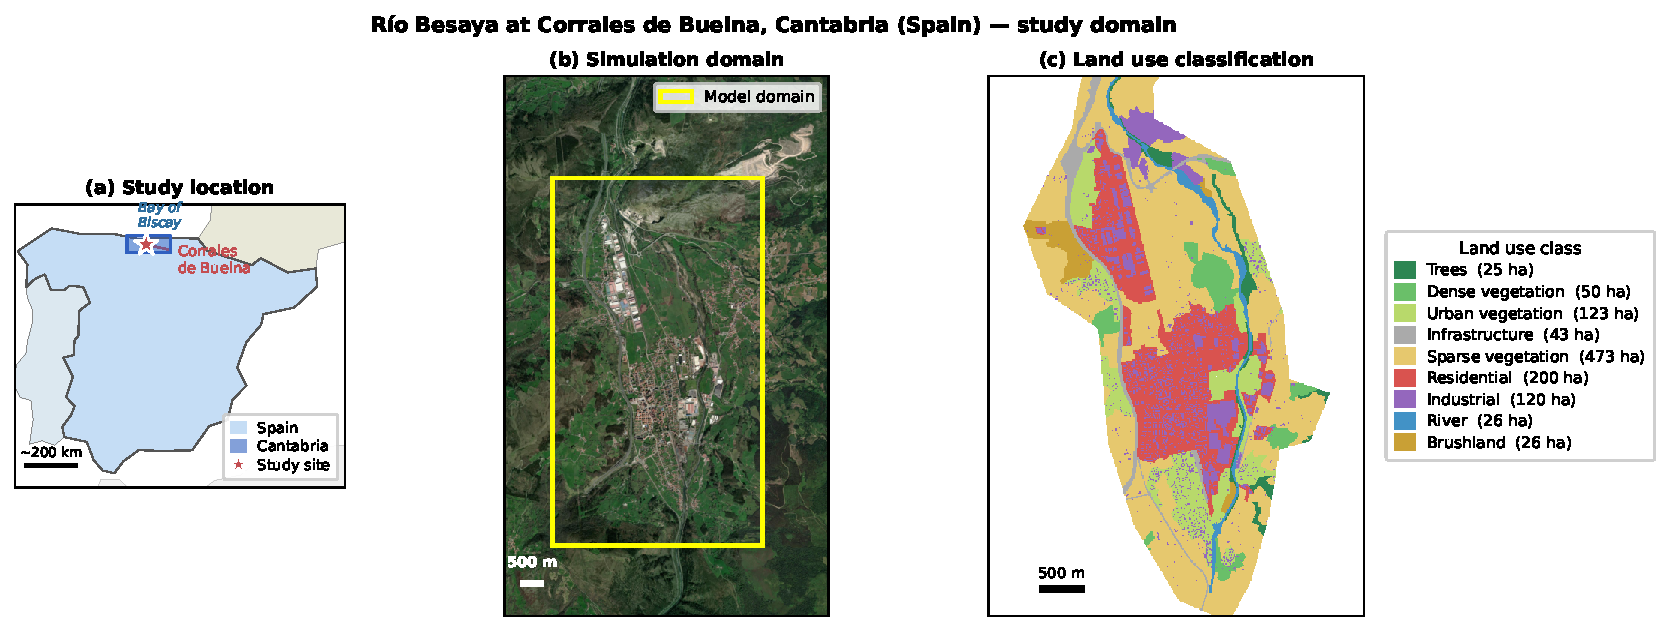
\includegraphics[width=\textwidth]{figures/fig00_location_map.pdf}
  \caption{Study area: Río Besaya at Corrales de Buelna, Cantabria, Spain.
    (a)~Regional context: Spain (light blue) with the autonomous community of
    Cantabria (blue shading) and the approximate course of the Besaya River
    (dark blue line); the red star ($\bigstar$) marks Corrales de Buelna
    ($\lambda = -4.052^{\circ}$, $\varphi = 43.238^{\circ}$, EPSG:4326).
    (b)~Satellite orthoimage of the simulation domain (ESRI World Imagery);
    the yellow rectangle delimits the 2D model extent
    ($\sim\!3.4 \times 6.0$~km, $\sim\!1\,086$~ha).
    (c)~Land use classification used to assign Manning roughness coefficients,
    derived from CORINE Land Cover 2018, reclassified into nine hydraulic
    classes and resampled to the 5~m model grid (ETRS89/UTM Zone~30N);
    nine classes are identified, with sparse vegetation (473~ha, 43.6\%)
    and residential areas (200~ha, 18.4\%) covering the largest fractions of the
    modelled domain.}
  \label{fig:location}
\end{figure}

\begin{figure}[htbp]
  \centering
  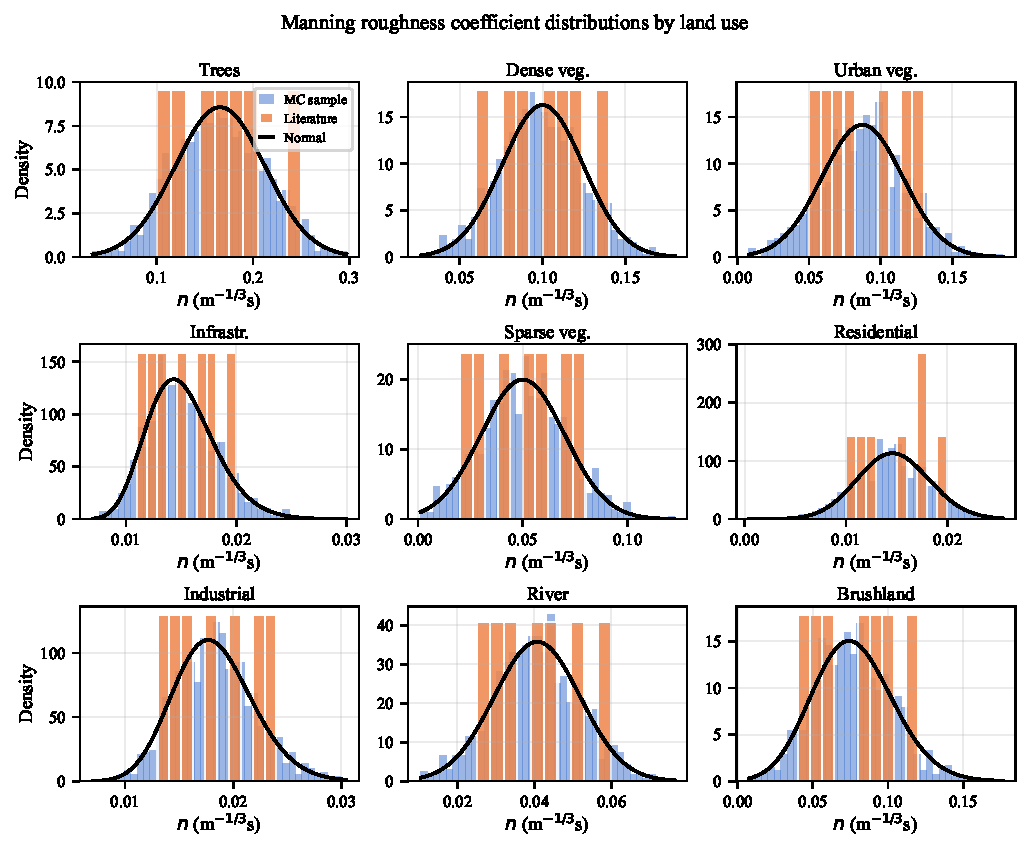
\includegraphics[width=\textwidth]{figures/fig01_manning_distributions.pdf}
  \caption{Fitted probability distributions (solid curves) for Manning's $n$
    in each land use class. Blue histograms: Monte Carlo samples ($N=1{,}000$);
    orange bars: bibliographic point values used as reference data.
    The distribution with the highest KS $p$-value is shown
    (Table~\ref{tab:manning}).
    The close agreement between the fitted PDF and the MC histogram indicates
    that the two-stage sampling procedure (pool of 10\,000; subsample of 1\,000)
    reproduces the intended parametric sampling distribution.}
  \label{fig:distributions}
\end{figure}

\begin{figure}[htbp]
  \centering
  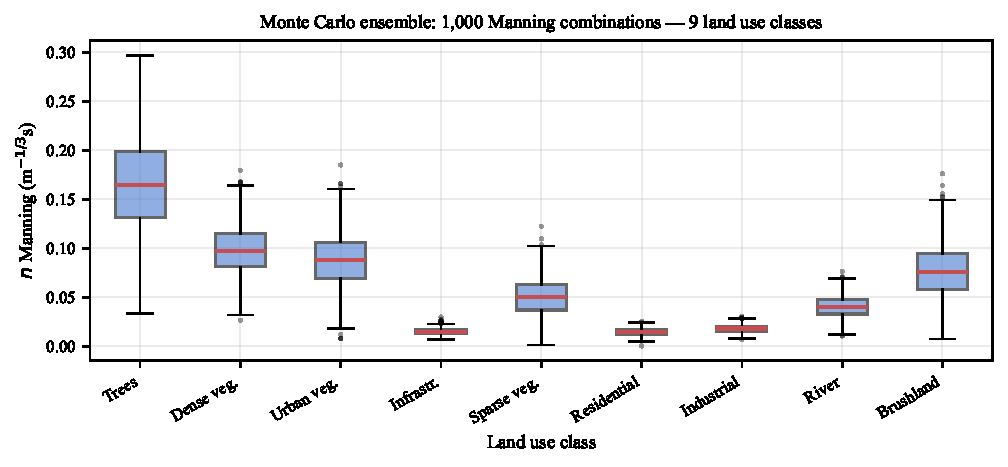
\includegraphics[width=\textwidth]{figures/fig02_mc_boxplots.pdf}
  \caption{Box plots of Manning $n$ across the 1\,000 Monte Carlo combinations
    for each land use class. Boxes: interquartile range (IQR); whiskers:
    $1.5 \times \mathrm{IQR}$; red line: median; circles: outliers.
    The median Manning values span approximately one order of magnitude
    across classes (0.015 to 0.165~m$^{-1/3}$s).
    The independent sampling of classes is intentional; no spatial or
    inter-class correlation is imposed.}
  \label{fig:mc_boxplots}
\end{figure}

\begin{figure}[htbp]
  \centering
  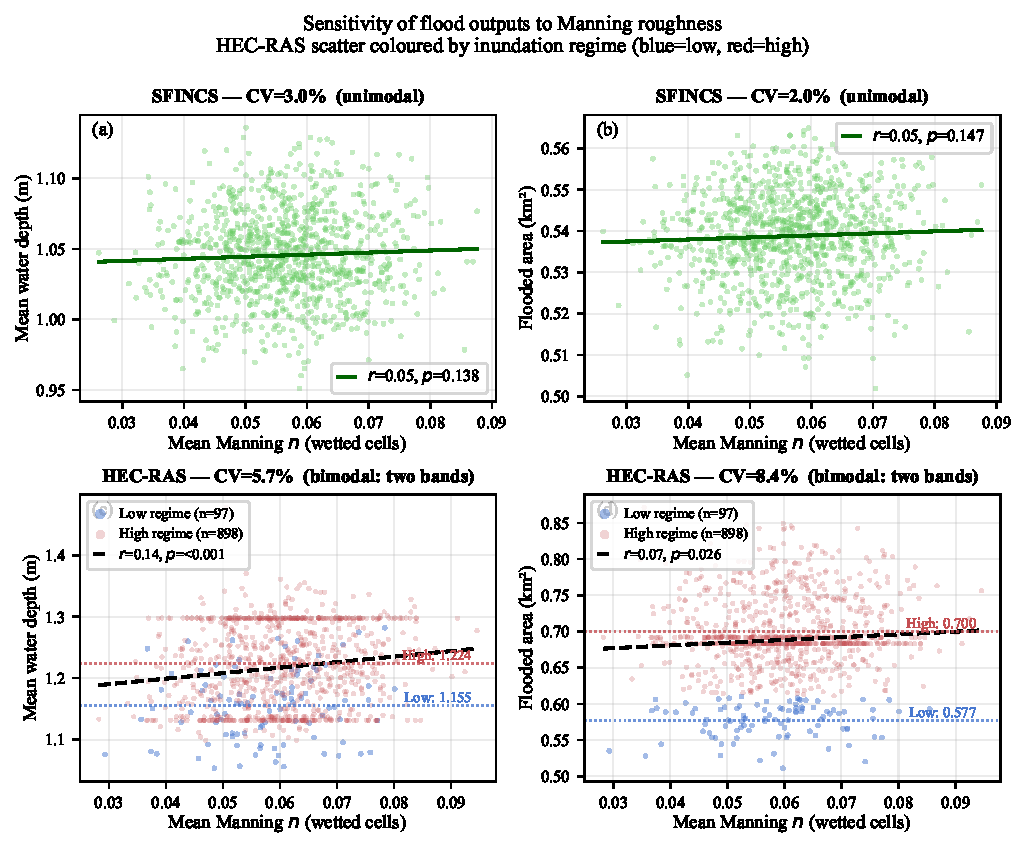
\includegraphics[width=\textwidth]{figures/fig03_intramodel_sensitivity.pdf}
  \caption{Scatter plots of mean water depth (left) and flooded area (right)
    versus spatially averaged Manning $n$ over wet cells, for \sfincs{}
    (top row, green) and \hecras{} (bottom row).
    In the \hecras{} panels (c--d), points are colored by the GMM-classified
    inundation regime: blue = low-area regime ($N = 97$ simulations,
    $\bar{A} = 0.577$~km\textsuperscript{2});
    red = high-area regime ($N = 898$, $\bar{A} = 0.700$~km\textsuperscript{2}).
    Horizontal dotted lines mark the mean of each band; the inter-band gap is
    $\Delta A \approx 0.124$~km\textsuperscript{2}.
    The two horizontal bands visible in panels (c--d) are not numerical
    artifacts but physically real inundation regimes (Section~\ref{sec:gmm}),
    driven by the simultaneous activation of a 7.4-ha secondary floodplain
    ($\sim$2\,960 cells) when the topographic saddle at 60.1~m a.s.l.\
    is overtopped (Section~\ref{sec:bifurcation}).
    Both bands span the full Manning range, confirming that roughness does
    not determine regime membership.
    Dashed regression lines and Pearson coefficients are computed on all
    995 simulations combined.
    CV values in panel titles refer to the coefficient of variation of the
    $y$-axis metric across all simulations.}
  \label{fig:sensitivity}
\end{figure}

\begin{figure}[htbp]
  \centering
  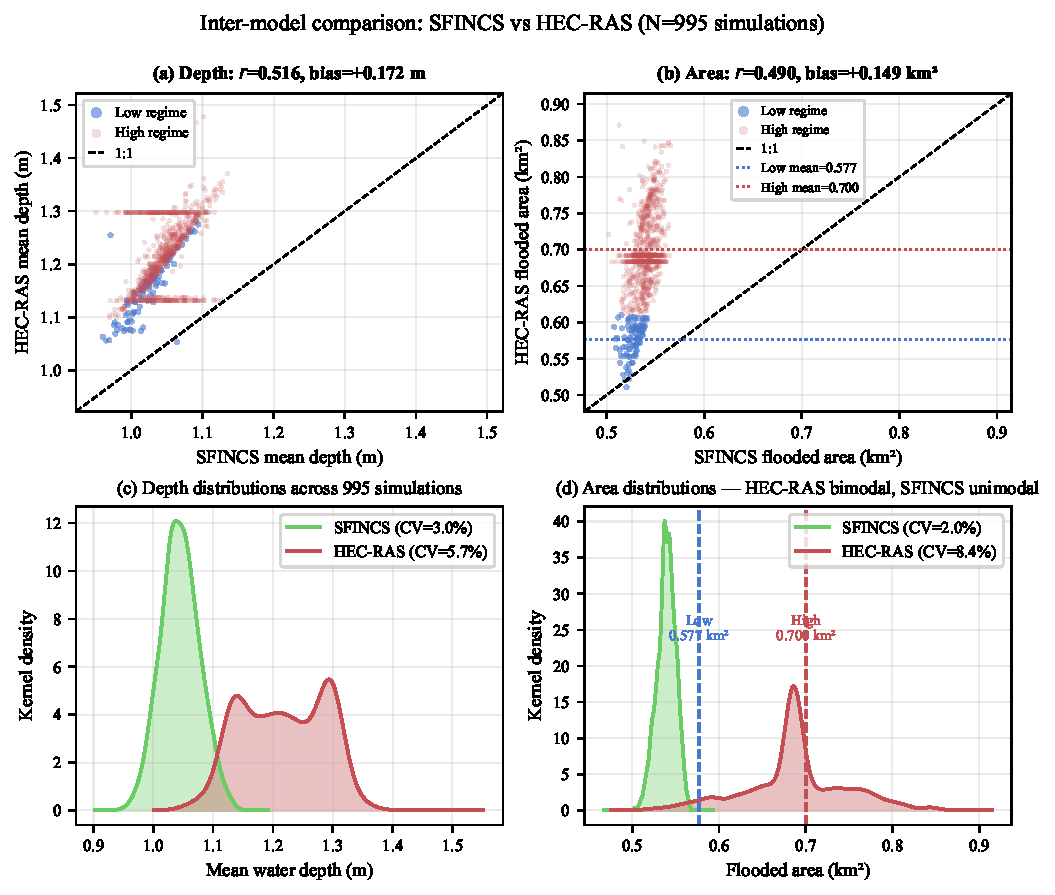
\includegraphics[width=\textwidth]{figures/fig04_intermodel_comparison.pdf}
  \caption{Inter-model comparison for 995 paired simulations.
    (a) 1:1 scatter of mean water depth (dashed line: perfect agreement);
    (b) 1:1 scatter of flooded area; horizontal dotted lines in (b) mark
    the band means of the low and high \hecras{} regimes.
    (c) Kernel density estimates of depth distributions across both models;
    (d) KDE of area distributions, showing the unimodal \sfincs{} response
    and the bimodal \hecras{} response; dashed vertical lines indicate the
    GMM component means.
    Points in (a--b) are colored by \hecras{} regime (blue: low; red: high).
    CV values in legend refer to the coefficient of variation of each model's
    ensemble.}
  \label{fig:comparison}
\end{figure}

\begin{figure}[htbp]
  \centering
  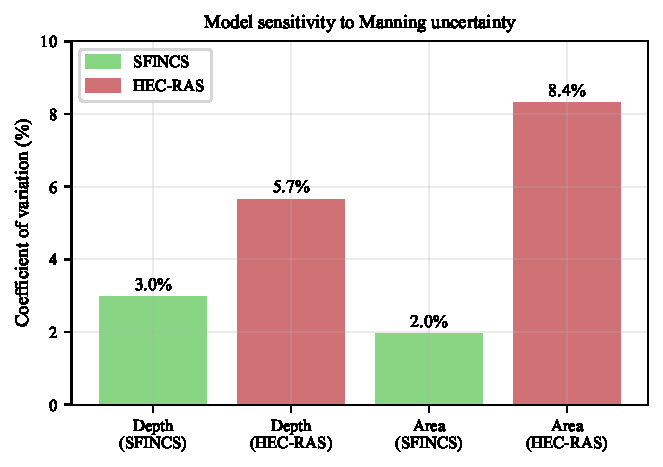
\includegraphics[width=\textwidth]{figures/fig06_cv_comparison.pdf}
  \caption{Coefficient of variation (CV) of mean water depth and flooded area
    for \sfincs{} (green) and \hecras{} (red) across 995 Monte Carlo
    simulations.
    \hecras{} is $1.9\times$ more sensitive than \sfincs{} for depth
    (CV: 5.7\% vs.\ 3.0\%) and $4.2\times$ more sensitive for area
    (CV: 8.4\% vs.\ 2.0\%).
    Values above bars show the CV to one decimal place.}
  \label{fig:cv}
\end{figure}

\begin{figure}[p]
  \centering
  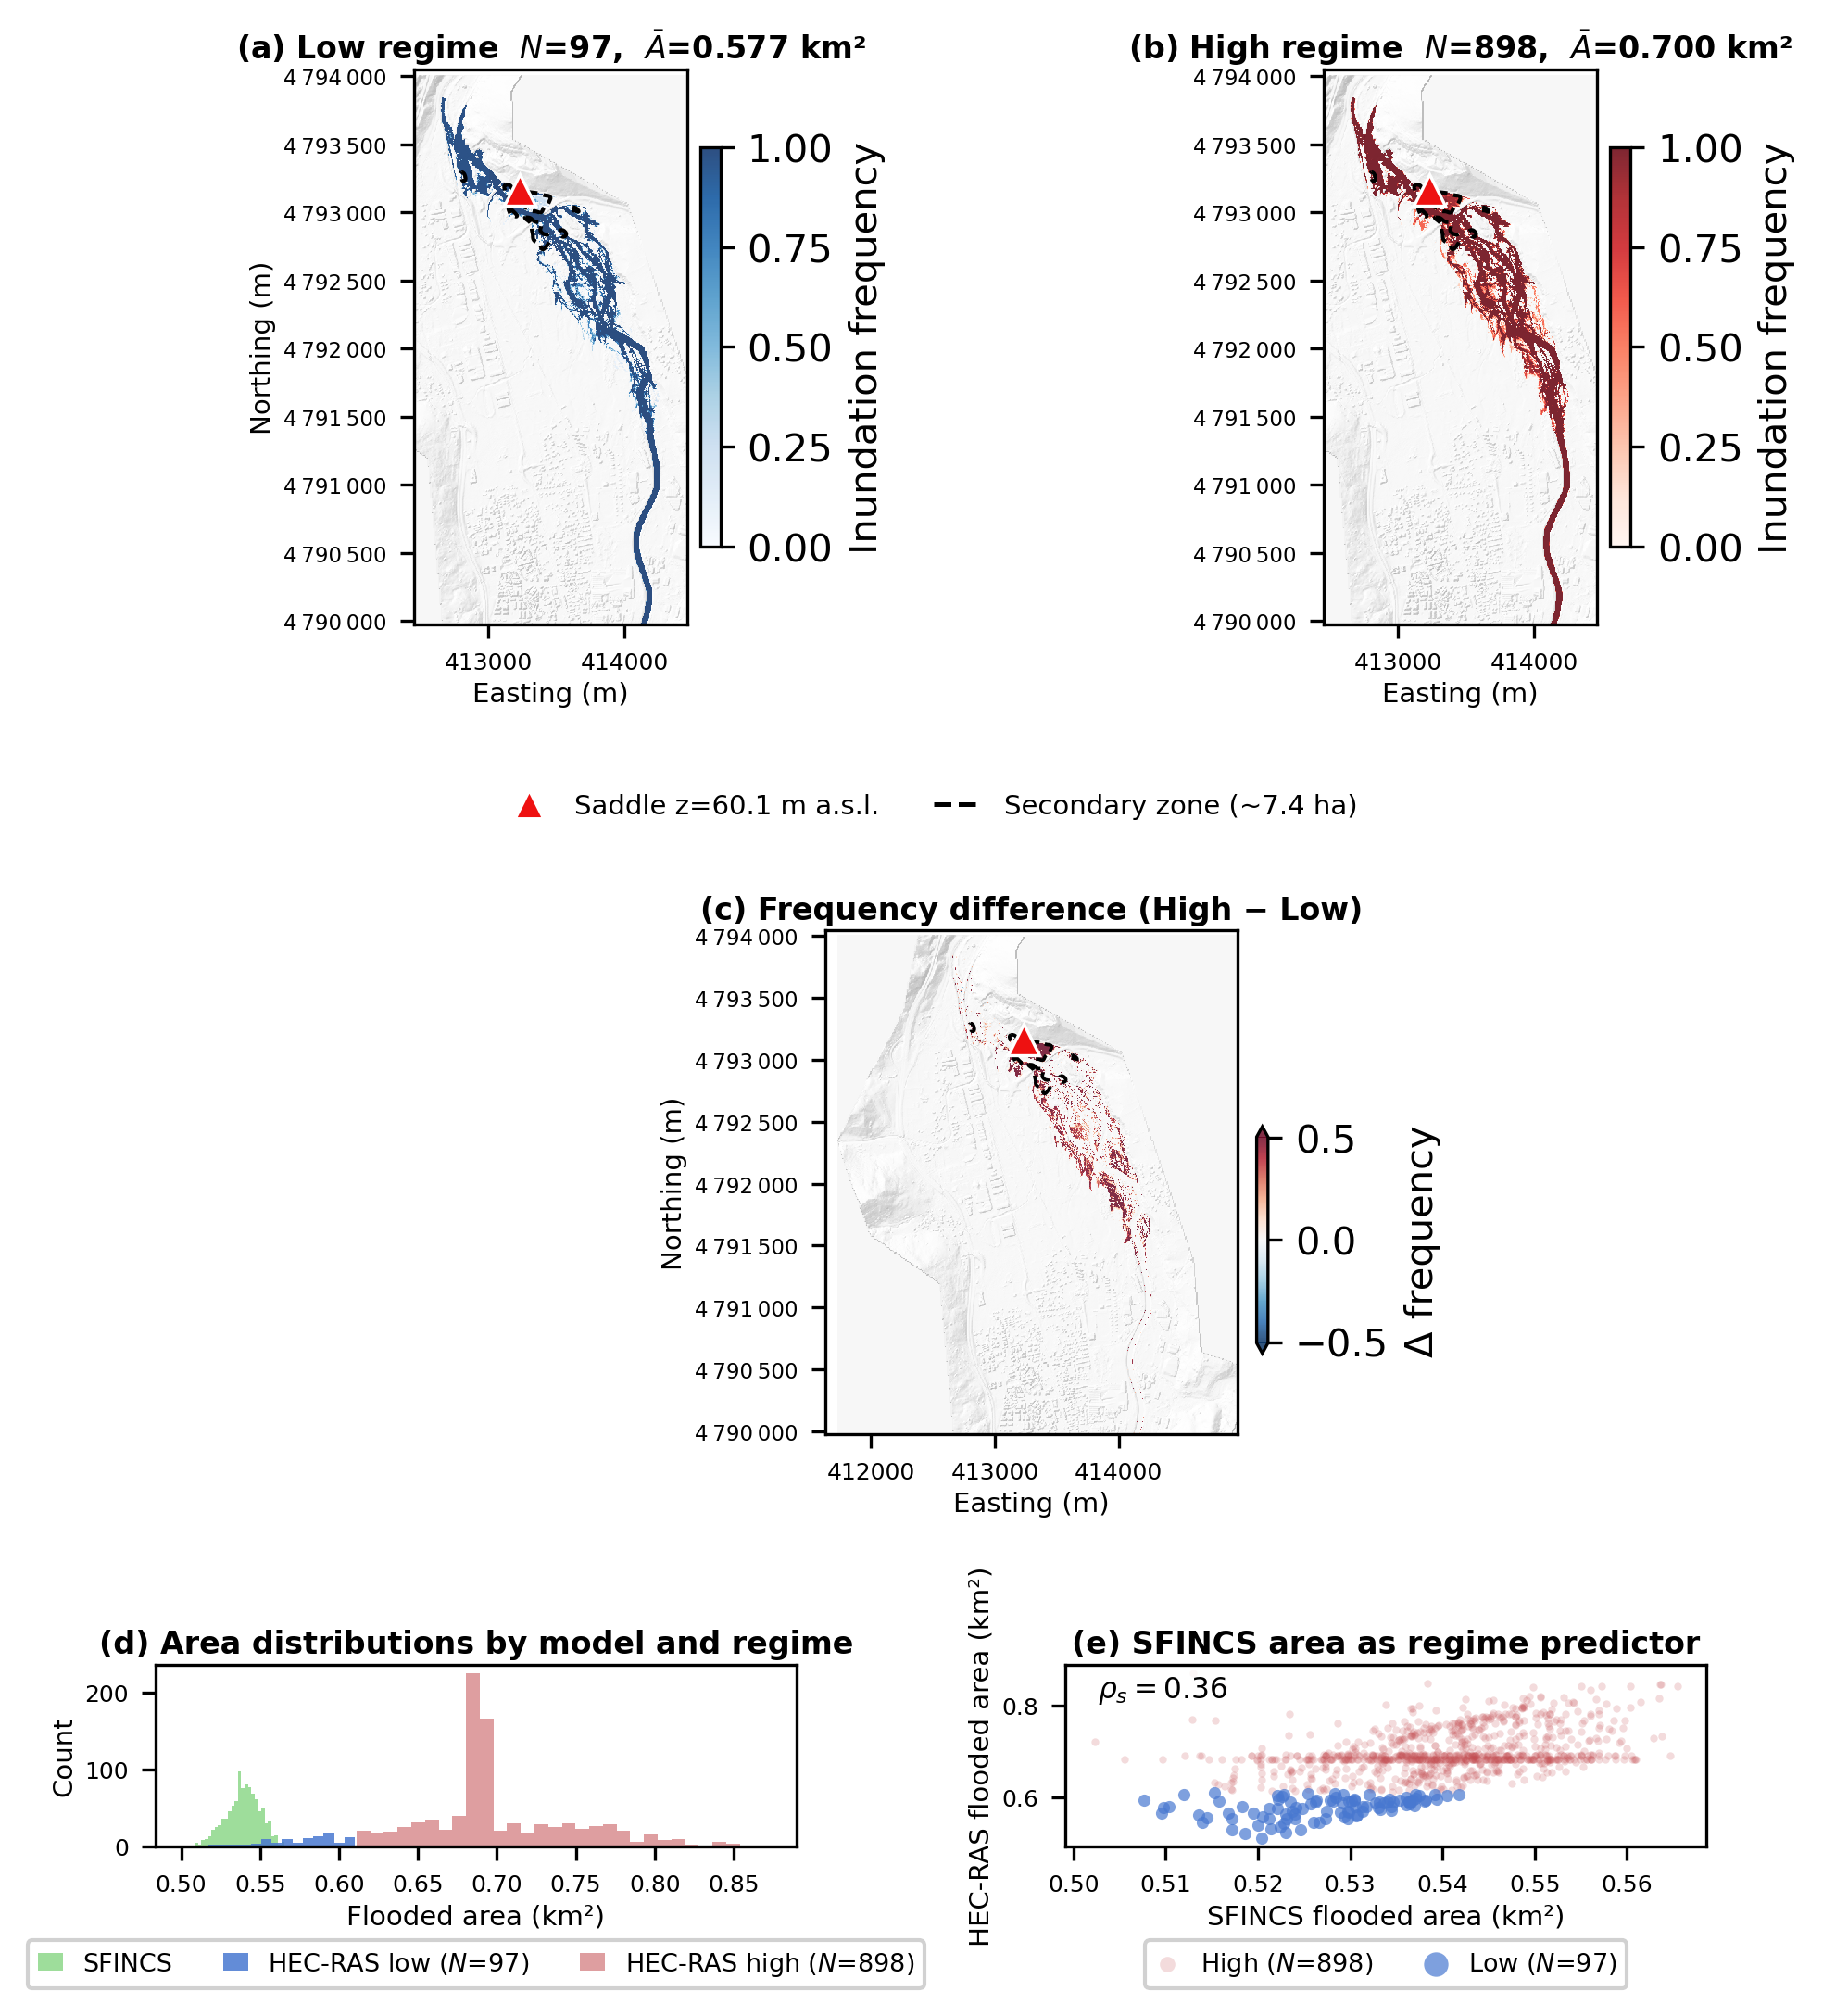
\includegraphics[width=\textwidth]{figures/fig05_hydraulic_bifurcation.pdf}
  \caption{Hydraulic bifurcation in \hecras{} at Corrales de Buelna.
    (a) Inundation frequency map for the low-area regime ($N = 97$
    simulations; blue scale);
    (b) frequency map for the high-area regime ($N = 898$; red scale).
    In both panels, the grey hillshade background shows local terrain relief;
    the dashed black contour encloses the secondary floodplain zone
    ($\Omega_\mathrm{secondary}$, $\sim 7.4$~ha) defined by
    Equation~(\ref{eq:omega}); and the red triangle ($\blacktriangle$)
    marks the topographic saddle at
    $z = 60.1$~m a.s.l.\ (X\,=\,413230, Y\,=\,4793166, EPSG:25830).
    (c) Frequency difference map (high $-$ low; red: cells exclusively
    wet in the high regime; blue: cells more frequently wet in the low regime).
    (d) Histogram of flooded areas for the two \hecras{} regimes and
    \sfincs{} (no bimodal structure visible in \sfincs{}).
    (e) \sfincs{} flooded area as a partial predictor of the \hecras{}
    regime (Spearman $\rho = +0.36$, $p < 10^{-31}$); lower \sfincs{}
    areas tend to correspond to the low \hecras{} regime, reflecting
    lower total flow energy in those simulations.}
  \label{fig:bifurcation}
\end{figure}

\begin{figure}[htbp]
  \centering
  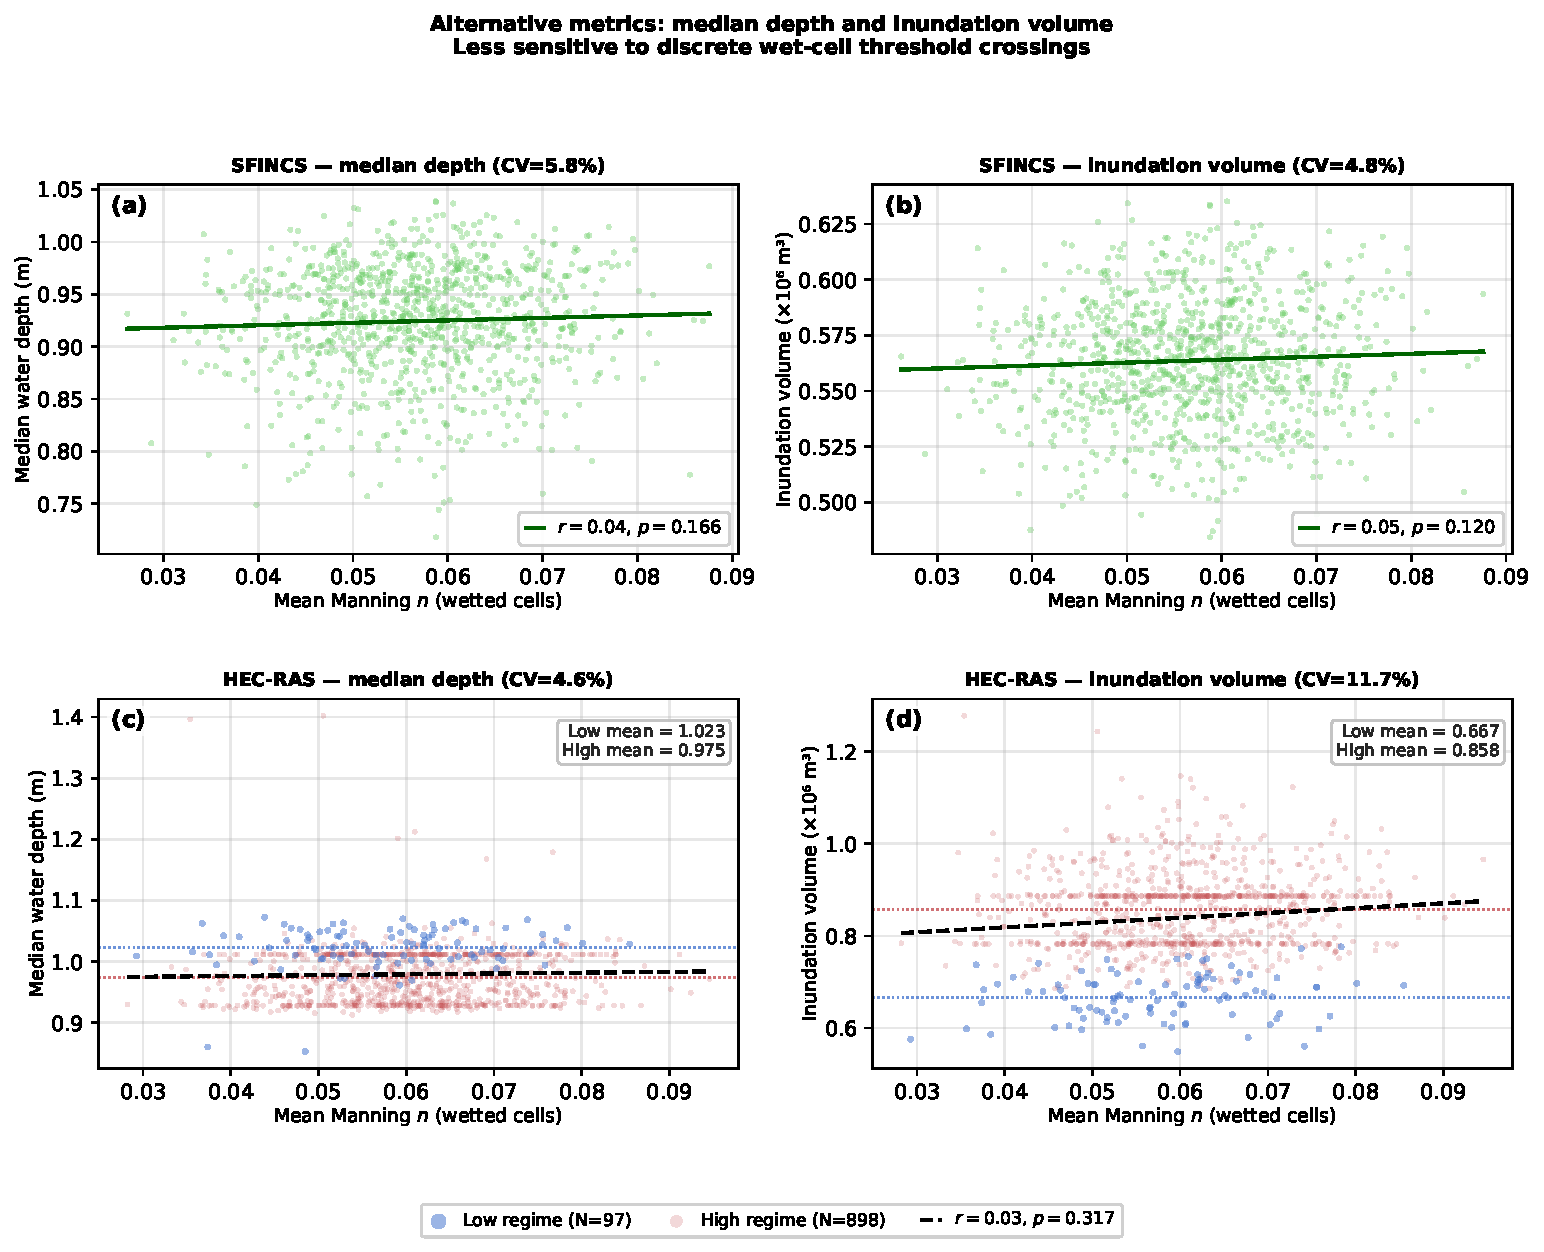
\includegraphics[width=\textwidth]{figures/fig07_alternative_metrics.pdf}
  \caption{Sensitivity scatter plots using alternative output metrics:
    median water depth $\tilde{h}$ (left column) and inundation volume $V$
    (right column) versus spatially averaged Manning $\bar{n}$ over wet cells,
    for \sfincs{} (top row, green) and \hecras{} (bottom row).
    \hecras{} points are colored by GMM regime (blue: low; red: high) as in
    Figure~\ref{fig:sensitivity}.
    Horizontal dotted lines mark the within-regime means of each metric.
    Dashed lines are OLS regression fits; CV values in panel titles are
    computed over all 995 simulations.
    The two-band structure persists in the volume scatter (d), confirming that
    the bimodality is a physical feature of the hydraulic response and not an
    artifact of the mean-depth metric.
    The inter-band gap is proportionally smaller in the volume scatter
    (Section~\ref{sec:alt_metrics}) because the newly activated
    near-threshold cells contribute negligible volume.
    Median depth (c) compresses the inter-band gap further because the
    median is less sensitive than the mean to a large influx of shallow cells.}
  \label{fig:alt_metrics}
\end{figure}

%% ===========================================================================
\clearpage
\section*{Supplementary Material}
\setcounter{figure}{0}
\setcounter{table}{0}
\renewcommand{\thefigure}{S\arabic{figure}}
\renewcommand{\thetable}{S\arabic{table}}

\paragraph{Robustness of main conclusions to inter-class Manning correlation.}
The following figures and table are provided as supplementary material to
support the independence-assumption sensitivity analysis described in
Section~\ref{sec:limitations}.
They are not part of the core narrative but document the analytical
robustness check in detail.

\begin{figure}[htbp]
  \centering
  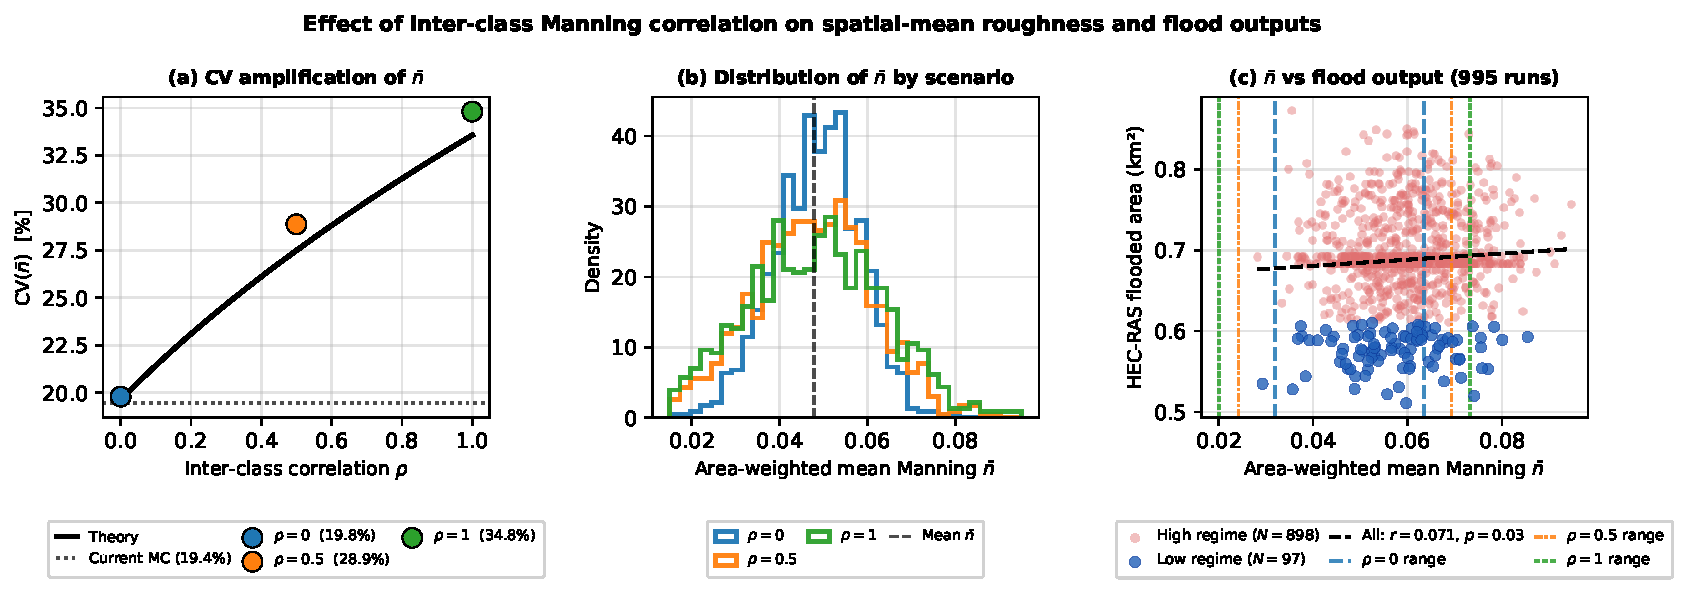
\includegraphics[width=\textwidth]{figures/fig_copula_analysis.pdf}
  \caption{Effect of inter-class Manning correlation on spatial-mean roughness
    and flood outputs ($N = 1\,000$ Gaussian copula samples per scenario).
    (a)~Theoretical CV amplification of the area-weighted mean Manning
    $\bar{n}$ with equi-correlation $\rho$ (solid curve); markers show
    empirical values; dotted line marks the reference independent-MC ensemble.
    (b)~Step histograms of $\bar{n}$: the distribution widens from
    CV\,=\,19.8\% ($\rho=0$) to 34.8\% ($\rho=1$) with no shift in the mean
    ($\bar{n}\approx 0.048$~m$^{-1/3}$s).
    (c)~$\bar{n}$ against HEC-RAS flooded area for 995 valid simulations
    coloured by hydraulic regime (upper-left legend: 5th--95th percentile
    range of $\bar{n}$ per scenario; lower-right legend: regime counts and
    regression); $r=0.071$ ($p=0.03$, $r^2<0.01$) shows only a weak direct
    association between inter-class Manning correlation and domain-scale
    flooded area; the regime fractions under correlated sampling are
    quantified in Supplementary Figure~S3.}
  \label{fig:copula}
\end{figure}

\begin{figure}[htbp]
  \centering
  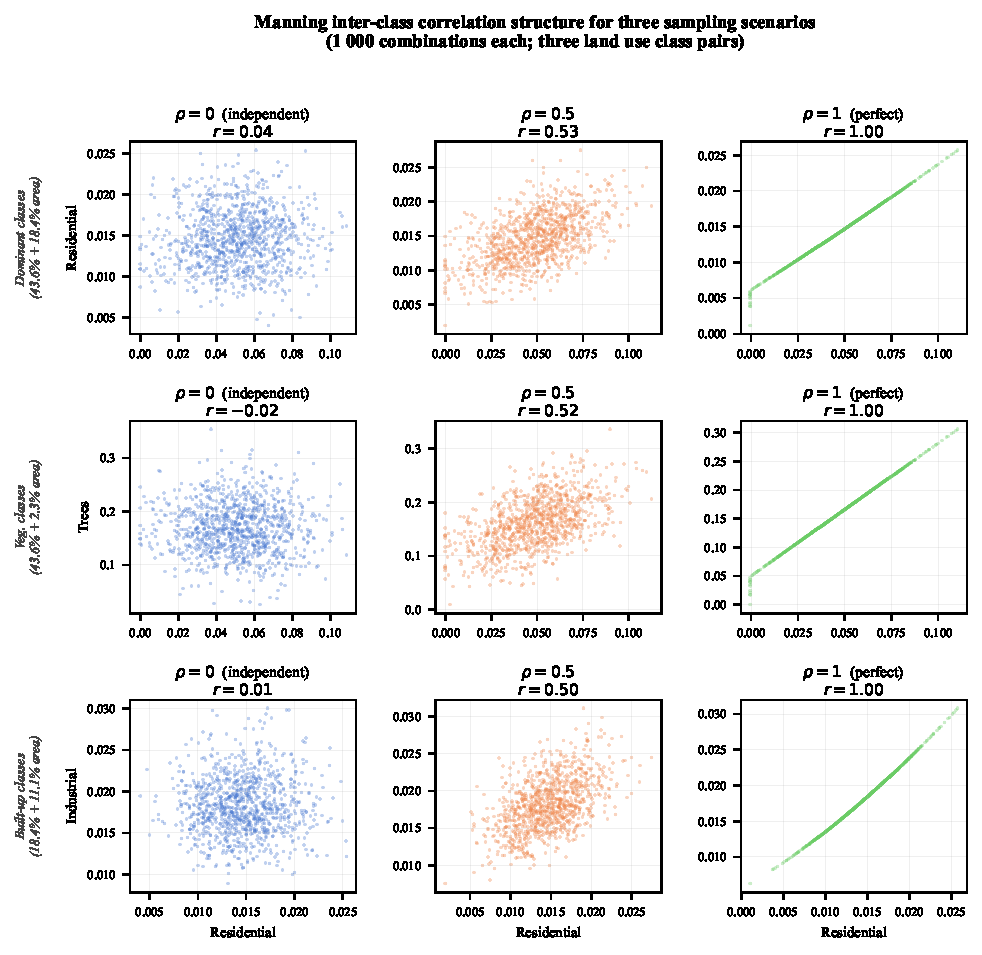
\includegraphics[width=\textwidth]{figures/fig_copula_scatter.pdf}
  \caption{Pairwise scatter plots of Manning $n$ values for three representative
    land use class pairs and three correlation scenarios
    ($N = 1\,000$ Gaussian copula samples each).
    Rows correspond to class pairs (dominant: sparse vegetation + residential;
    vegetation: sparse vegetation + trees; built-up: residential + industrial);
    columns correspond to equi-correlation values
    $\rho \in \{0,\,0.5,\,1.0\}$.
    Empirical Pearson $r$ confirms the copula reproduces the prescribed
    dependence structure.}
  \label{fig:copula_scatter}
\end{figure}

\begin{figure}[htbp]
  \centering
  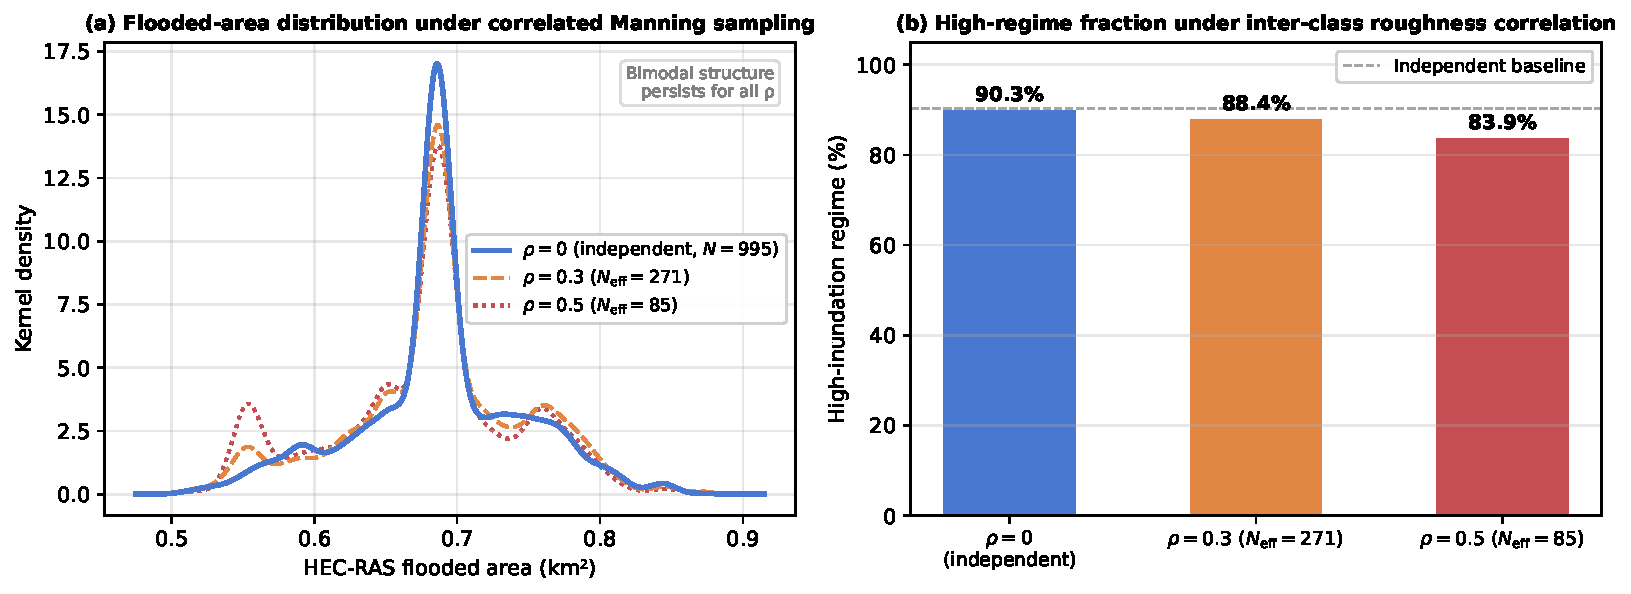
\includegraphics[width=\textwidth]{figures/fig_copula_is.pdf}
  \caption{Importance-sampling robustness check for inter-class Manning correlation.
    (\textbf{a})~Weighted kernel density estimates of \hecras{} flooded area
    under independent sampling ($\rho = 0$, $N = 995$) and two correlated
    scenarios ($\rho = 0.3$, effective $N = 271$; $\rho = 0.5$, effective $N = 85$).
    Weights are the ratio of the equicorrelation Gaussian copula density to
    the independent sampling density, computed from empirical probability
    integral transforms of the 9-class Manning vector.
    The bimodal structure of the \hecras{} response is preserved for all
    values of~$\rho$ shown.
    (\textbf{b})~High-inundation-regime fraction (weighted percentage) as a
    function of equicorrelation~$\rho$.
    The fraction decreases from 90.3\% (independent) to 88.4\% ($\rho = 0.3$)
    and 83.9\% ($\rho = 0.5$), confirming that the bimodal response is robust
    to plausible levels of inter-class roughness correlation.}
  \label{fig:copula_is}
\end{figure}

\clearpage
\begin{figure}[htbp]
  \centering
  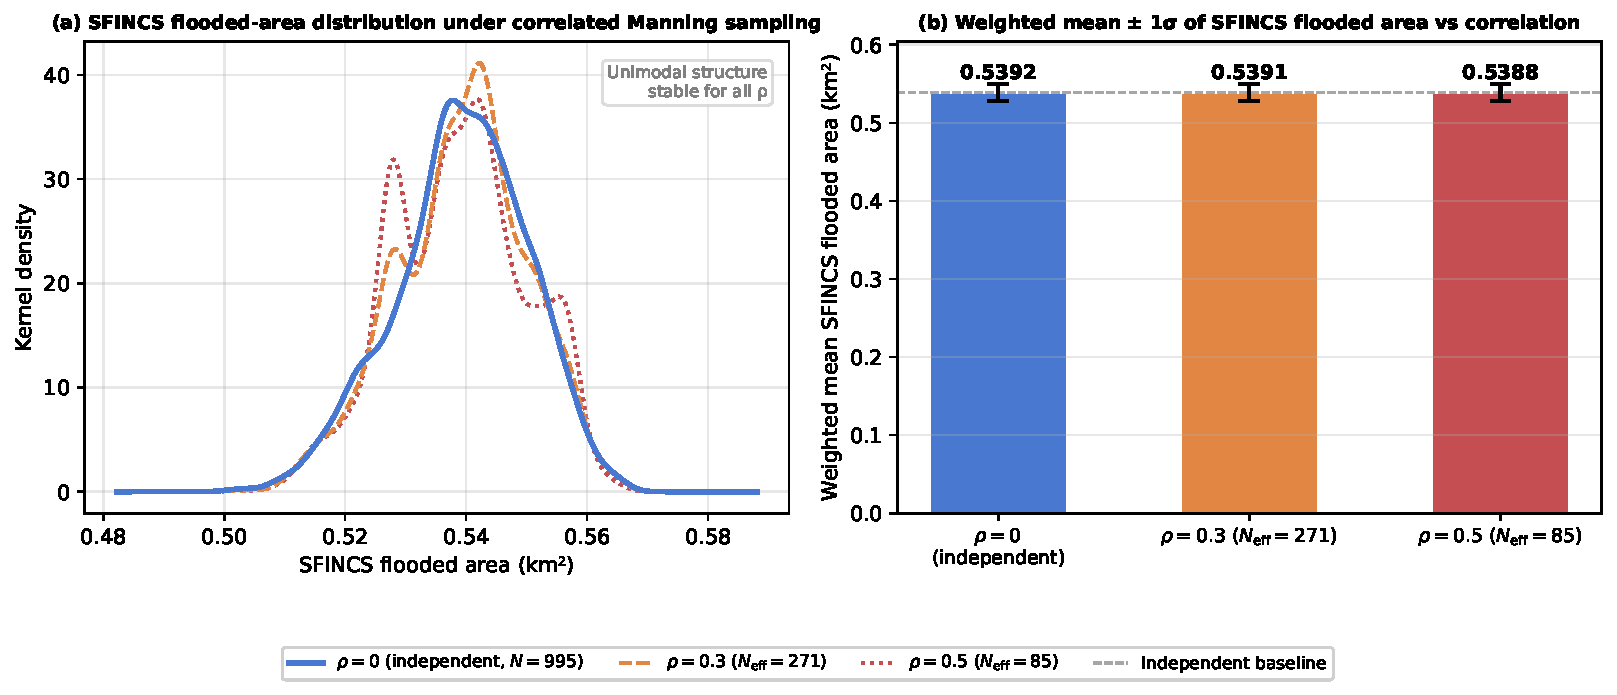
\includegraphics[width=\textwidth]{figures/fig_copula_is_sfincs.pdf}
  \caption{Importance-sampling robustness check for \sfincs{} under inter-class
    Manning correlation (counterpart to Supplementary Figure~S3 for \hecras{}).
    (\textbf{a})~Weighted kernel density estimates of \sfincs{} flooded area
    under independent sampling ($\rho = 0$, $N = 995$) and two correlated
    scenarios ($\rho = 0.3$, effective $N = 271$; $\rho = 0.5$, effective $N = 85$).
    The unimodal distribution is virtually unchanged across all values of~$\rho$.
    (\textbf{b})~Weighted mean $\pm1\sigma$ of \sfincs{} flooded area as a
    function of equicorrelation~$\rho$.
    The mean shifts by less than 0.1\% between $\rho = 0$ (0.5392~km$^2$) and
    $\rho = 0.5$ (0.5388~km$^2$), confirming that the unimodal \sfincs{}
    response is robust to plausible levels of inter-class roughness correlation.}
  \label{fig:copula_is_sfincs}
\end{figure}

\begin{table}[htbp]
  \centering
  \caption{Area-weighted spatial mean Manning $\bar{n}$ statistics under
    independent and Gaussian-copula correlated sampling
    ($N = 1\,000$ draws per scenario; domain area 1\,086~ha).
    P$_5$ and P$_{95}$ denote the 5th and 95th percentiles.}
  \label{tab:copula}
  \begin{tabular}{lcccccc}
    \hline
    Scenario & $\rho$ & Mean $\bar{n}$ & CV(\%) & P$_5$ & P$_{95}$ & P$_{95}$/P$_5$ \\
    \hline
    Independent (reference) & 0   & 0.0484 & 19.4 & 0.033 & 0.064 & 1.94 \\
    Copula $\rho = 0$        & 0   & 0.0486 & 19.8 & 0.032 & 0.063 & 1.98 \\
    Copula $\rho = 0.5$      & 0.5 & 0.0474 & 28.9 & 0.024 & 0.069 & 2.87 \\
    Copula $\rho = 1.0$      & 1.0 & 0.0474 & 34.8 & 0.020 & 0.073 & 3.66 \\
    \hline
  \end{tabular}
\end{table}

\begin{landscape}
\begin{table}[htbp]
  \centering
  \caption{\textbf{Simulations removed prior to analysis} ($N = 5$, 0.5\% of 1\,000).
    Anomalies were detected using a robust $z$-score with threshold
    $k = 5$ (see Section~\ref{sec:cleaning}).
    Model: S\,=\,SFINCS; H\,=\,HEC-RAS.
    SFINCS outputs for all five simulations lie within the normal ensemble
    range, indicating that the anomalies are model-specific non-convergences
    not attributable to extreme Manning combinations.
    Ensemble medians for reference: HEC-RAS area $\approx 0.668$~km$^2$,
    depth $\approx 1.22$~m; SFINCS area $\approx 0.537$~km$^2$,
    depth $\approx 1.04$~m.}
  \label{tab:anomalous}
  \small
  \begin{tabular}{cclp{2.4cm}ccccc}
    \toprule
    Sim. & Model & Flagged metric & Flagged value & $|z|_{\mathrm{robust}}$ &
    \multicolumn{2}{c}{HEC-RAS output} & \multicolumn{2}{c}{SFINCS output} \\
    \cmidrule(lr){6-7}\cmidrule(lr){8-9}
    & & & & & Area (km$^2$) & Depth (m) & Area (km$^2$) & Depth (m) \\
    \midrule
    29  & H & Mean depth   & 1.930~m        & 6.70 & 2.187 & 1.930 & 0.498 & 0.949 \\
    295 & H & Mean depth   & 1.772~m        & 5.21 & 1.664 & 1.772 & 0.499 & 0.948 \\
    633 & S & Flooded area & 0.467~km$^{2}$ & 6.84 & 0.865 & 1.545 & 0.467 & 1.005 \\
    724 & H & Mean depth   & 1.805~m        & 5.52 & 1.118 & 1.805 & 0.512 & 0.994 \\
    755 & H & Mean depth   & 1.834~m        & 5.79 & 1.865 & 1.834 & 0.503 & 0.962 \\
    \bottomrule
  \end{tabular}
\end{table}
\end{landscape}

\end{document}
